\chapter{Object Reconstruction}
\label{chap:reconstruction}


\section{Introduction}
\label{reco:sec:intro}

This chapter deals with the way in which the simulation and the data collected at the \CMS experiment are processed for use in the \Hgg analysis. The reconstruction is performed using custom-built software: parts of the processing which are common to most \CMS analyses are performed using the \CMSSW package; further reconstruction which is specific to the \Hgg analysis is performed using the \FLASHgg software. %The \CMSSW software uses the \PF algorithm, in which energy deposits from the various sub-detectors are combined to reconstruct individual particles. This algorithm is described in \Sec~\ref{reco:sec:pf}. The reconstruction and identification of particles often uses \MVA techniques, known as \BDT\s, which are described in \Sec~\ref{reco:sec:bdt}. 
A short discussion on some of the methods which are used to perform and validate the reconstruction of particles can be found in \Sec~\ref{reco:sec:tools}. 
The same reconstruction algorithms are applied both to the data collected at the \CMS experiment and to simulated samples. % where the interaction of generated particles with the \CMS sub-detectors is simulated. The way in which both data and simulation are obtained are described in \Sec~\ref{th:sec:samples}.
The way in which both types of sample is obtained is discussed in \Sec~\ref{reco:sec:samples}.

The work presented in this thesis involves the study of the Higgs boson decaying to photons, \Hgg. It has already been noted in \Sec~\ref{th:sec:higgs_decays} that \Hgg is one of the most sensitive decays with which the Higgs boson can be observed and its properties measured in the \LHC environment. This is despite it having a small branching fraction ($\sim 0.2\% $) and an irreducible \SM background of \QCD processes which have two photons in the final state. The channel has the benefit of having a fully reconstructible final state and a clean signature. The experimental method to study the Higgs boson is therefore to look for a resonant Higgs boson peak on top of a continuous diphoton invariant mass spectrum.
It can be shown that the invariant mass of the diphoton system (\mgg), i.e. the invariant mass of the Higgs boson, is given by:
\begin{equation}
\label{reco:eq:mgg}
 \mgg = \sqrt{2 E_{\gamma}^1 E_{\gamma}^2 (1-\cos\alpha)}, 
\end{equation}

where $E_{\gamma}^{1,2}$ represent the energies of the two photons and $\alpha$ represents the opening angle between them. The calculation of opening angle relies on identifying the spatial location of the Higgs boson decay. Therefore, \Eq~\ref{reco:eq:mgg} indicates that to study \Hgg, the most important steps are the reconstruction of photons and location of the \PV. These two steps are discussed in \Sec~\ref{reco:sec:photons} and \Sec~\ref{reco:sec:vertex} respectively. 

Higgs bosons are produced at the \LHC chiefly by the mechanisms, or \emph{modes}, described in \Sec~\ref{sec:th:higgs_production_modes}. At leading order, in the dominant production mode, \ggH, the final state consists only of the two Higgs decay photons. However, for other production modes, the Higgs boson can be produced in association with other particles. These additional objects in the detector can be reconstructed and provide information on the mode in which the Higgs boson was likely to have been produced. The methods used to reconstruct such additional objects are described in \Sec~\ref{reco:sec:other}.

\section{Common reconstruction methods}
\label{reco:sec:tools}

Some analysis methods occur repeatedly throughout the reconstruction process. A short description of these techniques is given here. 

\subsection{Particle-flow}
\label{reco:sec:pf}

The \PF event reconstruction algorithm~\cite{CMS-PAS-PFT-09-001,CMS-PAS-PFT-10-001} combines information from all \CMS \subdetector\s to reconstruct and identify individual particles. The inputs to this algorithm are the tracks reconstructed in the tracker and muon system, and the clusters of energy deposits in the \ECAL and \HCAL. The outputs of the algorithm are objects corresponding to stable particles (photons, electrons, muons, charged hadrons or neutral hadrons). These so called \PF \emph{candidates} can then be further clustered to obtain jets. In this scheme, \ECAL \SC\s which are not on the extrapolated trajectory of tracks from either the muon system or the tracker are identified as photon candidates. If a charged particle track in the tracker is associated to one or more \ECAL \SC\s (corresponding to the main electron and photons radiated by bremsstrahlung), then it can be identified as an electron electron candidate. If a track in the tracker consistent with a track or multiple hits in the muon system, then it is identified as a muon candidate. Tracks in the tracker which are not associated with any track in the muon system or any deposit in the \ECAL are interpreted as charged hadron candidates. Finally, deposits in the \HCAL which are not associated with any tracks, or which are in excess of the expected \HCAL energy from another \PF particle, are identified as neutral hadron candidates.

\subsection{Boosted Decision Trees}
\label{reco:sec:bdt}

Analyses in \HEP often use \MVA techniques to improve their overall sensitivity. An example of an \MVA technique which is used repeatedly in this thesis is the \DT method, where a technique known as \emph{boosting} is applied to produce a \BDT. Problems where a \BDT is of use always involve a list of items with $N_{\textrm{inputs}}$ \emph{features} or \emph{input variables}, labelled here $\vec{x} =(x_0, ... ,x_{N_{\textrm{inputs}}})$, and a property $y$, the \emph{target variable} which is to be determined. The objective of a \BDT is to produce a function $F(\vec{x})$ which is an estimate of the true value of $y$ for a given set of input variable values~\cite{friedman2001}. There are two common uses for \BDT\s: \emph{classification} and \emph{regression}. For example, in many classification \BDT\s used in this thesis, the items are events, and $y$ describes whether an  event contained a Higgs boson decay (signal-like) or not (background-like), based on a set of input variables $\vec{x}$ derived from properties of the \PF objects in the event. In this example, as with all classification \BDT\s, the target variable takes discrete values (background-like or signal-like). In the case of regression \BDT\s, the target variable is  continuous rather than discrete. For example, the energy correction ($y$ is $F_{\text{SC}}$ in \Eq~\ref{eq:cms:ecal:energy}) for \SC\s in the \ECAL is obtained using a regression \BDT, as is described in \Sec~\ref{recp:sec:photon_energy_correction_bdt}. The \BDT\s used in this thesis were trained using the \TMVA framework~\cite{TMVA} as part of the \ROOT software package. 

In general, a \BDT is a linear combination of \DT\s. A \DT is obtained using a \emph{training dataset} consisting of a list of $N_{\textrm{items}}$ items $(\vec{x}_{m},y_{m},w_{m})$ for $m=0,...,N_{\textrm{items}}$, where for each item, $\vec{x}_{m}$ is a set of input variables values and $y_{m}$ is the true value of the target variable. The items can be weighted with weight $w_{m}$. In the simplest case, the value of $y_{m}$ is binary for any given $m$: signal or background. A numerical value, $1$ and $-1$ say, can be assigned to these two options respectively. The following description uses this binary output example, but can be generalised for $y_{m}$ to be able to be assigned any number of discrete values for classification \DT\s, or continuous values in the case of regression \DT\s.
In order to construct a \DT, the training dataset is first split into two sub-samples by applying a selection on one or more of the input variables, which will be referred to as a \emph{cut}. The \emph{purity} $p^{\textrm{subsample}}$, which is simply the proportion of signal-like items in a sub-sample, is given by:

\begin{equation}
 p^{\textrm{subsample}} = \frac{\sum_{m=0}^{N_{\textrm{items}}^{\textrm{subsample}}} w_{m} \textrm{Bool}(y_m=1)}{\sum_{m=0}^{N_{\textrm{items}}^{\textrm{subsample}}} w_{m}}, 
\end{equation}

where $\textrm{Bool}(X)$ is equal to $1$ $(0)$ if $X$ it true (false). 
The cuts on the input variables are chosen in order to maximise the separation of signal and background in the resulting sub-samples. This is achieved by minimizing a separation criterion. 
A common separation criterion is the \emph{Gini index} $2p^{\textrm{subsample}}(1-p^{\textrm{subsample}})$, which has a maximum at $0.5$ for sub-samples with an equal amount of signal and background items and gives $0$ in cases where all items are of the same type (signal or background). Many other separation criteria exist, for instance \emph{cross-entropy, misclassification error, statistical significance} and \emph{average squared error}.  
Each sub-sample can then be further split by a new set of cuts on the target variables. This procedure is repeated iteratively for each sub-sample until either the number of iterations reaches some predefined threshold known as the \emph{tree depth}, or if the sub-sample satisfies some predetermined requirement on the value of the separation criterion. Each sub-sample obtained after the final set of cuts has been applied is known as a \emph{leaf}. The output score of the items in a given leaf is then $1 (-1)$ if $p^{\textrm{subsample}}>0.5$ $(p^{\textrm{subsample}}\leq0.5)$.

The procedure known as boosting helps to improve the performance of a \DT, for example by reducing the impact of statistical fluctuations in the training sample. Many boosting algorithms exist, but in all cases several individual \DT\s are produced, each trained on subsets or modified versions of the training dataset. The final \BDT is a weighted linear combination of the individual \DT\s. Supposing that there are $N_{\textrm{DT}}$ individual \DT\s, labelled as $f_{l}(\vec{x},\vec{\alpha}_{l})$ where $l=0,..,N_{\textrm{DT}}$ and $\vec{\alpha}_{l}$ is the set of cuts in the corresponding \DT, the full \BDT, $F$, is written as:

\begin{equation}
\label{reco:eq:bdt}
F(\vec{x},\vec{\beta},\vec{\alpha}) = \sum_{l=0}^{N_{\textrm{DT}}} \beta_{l} f_{l}(\vec{x},\vec{\alpha_{l}}), 
\end{equation}

where $\vec{\beta}=(\beta_{0},...,\beta_{N_{\textrm{DT}}})$ is the set of coefficients applied to each \DT in the \BDT. The values of of $\vec{\beta}$ are determined by the boosting algorithm used~\cite{friedman2009,TMVA}. A consequence of \Eq~\ref{reco:eq:bdt} is that the output of the \BDT is no longer a discrete value of $\pm1$, but instead a semi-continuous variable between -1 and 1. 

Some of the most common boosting algorithms are \emph{adaptive boosting} and \emph{gradient boosting}. In adaptive boosting, the first \DT is trained on the full training dataset as usual. The training dataset is then re-weighted so that items which were assigned an incorrect output score by the previous \DT are given a larger weight and the items which were correctly classified are given a smaller weight. The next \DT is then trained on the modified dataset, and the whole procedure is repeated over a large number of iterations. The final $\vec{\beta}$ for adaptive boosting algorithms is given by the logarithm of the weights applied to the dataset at each step. In gradient boosting, for the $N_{\textrm{DT}}$ \DT\s in \Eq~\ref{reco:eq:bdt}, the values of the individual components of $\vec{\alpha}$ and $\vec{\beta}$ are varied in such a way as to minimise the \emph{loss function} $L(F,y)$, which is a measure of the deviation of the \BDT output $y = F(\vec{x},\vec{\beta},\vec{\alpha})$ from the true value $y^T$ across all items in the training dataset. Popular choices for the loss function include $L(F,y) = ( y - F(\vec{x},\vec{\beta},\vec{\alpha}))^2$ and  $L(F,y) = \ln (1 + e^{-2F(\vec{x},\vec{\beta},\vec{\alpha})y})$~\cite{friedman2009,TMVA}.

\subsection{Tag-and-probe}
\label{reco:sec:tagandprobe}

The \TagAndProbe technique~\cite{TagAndProbe} is a common way to determine the efficiency of a selection $S$ in data. The technique exploits decays where a resonant particle decays to a pair of particles, for instance \Zee or \Zmumu. The events used for the tag-and-probe are selected such that the invariant mass of the decay products are near the mass peak of the resonant particle, thus ensuring a fairly pure sample. One can then impose a strict identification requirement on one of the decay products, which is refereed to as the \emph{tag}, and then apply a very loose identification requirement for the other decay product, referred to as the \emph{probe}. The requirements applied to the probe should be loose enough that they does not affect the efficiency of $S$. The efficiency of $S$ is then the fraction of probe decay particles which satisfy $S$. 

\section{Samples}
\label{reco:sec:samples}
\subsection{Simulation samples}

\emph{Signal samples} are sets of simulated events containing \Hgg decays, which are produced for each of the main Higgs boson production modes, each for a range of values of \mH. The cross-section and branching fractions used for the simulation under each \mH scenario are those recommended by the \LHCHXSWG~\cite{LHCHXSWGYR4}. Signal samples are used to train \BDT\s, validate reconstruction algorithms and produce signal models, as described in \Sec~\ref{stat:sec:signal_model}. Signal simulations are produced at parton-level using the generator \Madgraph~\cite{Madgraph}, which makes use of perturbative \QCD at \NLO. The parton-level samples are then interfaced with \Pythia~\cite{Pythia8}, using the tune \PythiaTune~\cite{PythiaTune}, which models the subsequent showering and hadronisation of partons. 
\emph{Background samples} are sets of events which represent the reducible and irreducible backgrounds for the \Hgg decay. As for the signal samples, these are used to train \BDT\s, to validate reconstruction algorithms and to optimise the categorisation scheme. However, the background model, described in \Sec~\ref{stat:sec:background_model}, does not use simulated samples, and is instead derived directly from data. The \emph{irreducible background} samples are composed of \SM processes which yield genuine photons from a \pp interaction in the final state, and are modelled using the \Sherpa~\cite{Sherpa} generator. The \emph{reducible background} samples represent events where jets are incorrectly identified as isolated photons. The largest contributors to the reducible background are \gammaJet and \QCDmultijet events, which are modelled using the \Pythia generator, where a filter designed to enhance the fraction of events with a large component of electromagnetic energy was applied. %The filter required a potential photon signal (photon, electron, or neutral hadrons, with $pt>15 \GeV$
\DY, \Wg and \Zg samples are also used for validation purposes, and these are simulated using \Madgraph. 

For all simulated samples, the detailed response of the \CMS detector is modelled using \Geant~\cite{Geant}, which takes into account \PU effects in the nominal bunch crossing as well as in previous and subsequent bunch crossings. The samples are re-weighted such that their \PU distributions match those observed in data before they are used in the analysis.

\subsection{Data samples and trigger} % including triggers
\label{sec:reco:data}

The data sample analysed in this thesis was recorded using the \CMS detector in between March and October 2016, during \pp LHC collisions at $\sqrt{s}=13\TeV$. It corresponds to an integrated luminosity of \totaldatatwentysixteen\ifb. As was described in \Sec~\ref{detector:sec:trigger}, events which are recorded for analysis at \CMS must pass the requirements of the triggering system. 

The \LI requires either a deposit in the \ECAL with $\pT>25\GeV$ or two deposits with $\pT>15\GeV$ and $\pT>10\GeV$ respectively. Events passing the \LI are processed at the \HLT, where a basic clustering is applied to the candidate photon deposits. The requirements for an events to be saved to the double-photon sample by the \HLT are as follows:

%such as the invariant mass of diphoton pairs (\mgg), the transverse energy of candidate photons \ET and the  \RNINE of a candidate, For an event to be saved in the double-photon sample, the trigger requires:
\begin{itemize}
\item the event contains two candidate photons, with \mgg above 90\GeV,
\item the candidate photon with most energy satisfies $\ET >30\GeV$, 
\item the candidate photon with second-most energy satisfies $\ET >18\GeV$,
%\item the two candidate photons must either have a large value of \RNINE (defined as the sum of the energy of the $3\times3$ array of crystals around the most energetic crystal in a \SC, divided by the energy of the \SC) or pass a loose calorimeter-based identification and isolation requirement.
\item both candidate photons pass a loose calorimeter-based identification using shower shape and isolation requirements.
\end{itemize}

Events passing the \LI and \HLT requirements detailed in \Sec~\ref{sec:reco:data} are saved for further processing. The efficiency of the trigger requirements was studied using a modified \TagAndProbe method in data using \Zee events. The \LI efficiency is found to be above 97.5\% in the \EB and above 92\% in the \EE. The efficiency of the \HLT is found to be above 97\% in the \EB and 96\% in the \EE. %The \Zee data sample is obtained using a special trigger which relies on loose requirements on a single electron. Using an additional selection on the invariant mass of events with two electrons, it is possible to select a high-purity \Zee sample using this trigger. The electrons are reconstructed as photons and passed through the reconstruction steps detailed in this chapter.  


\section{Photon reconstruction} 
\label{reco:sec:photons}




\subsection{Clustering of \ECAL deposits}

The most important \subdetector for the reconstruction of photons is the \ECAL. Photons or electrons which impact the \ECAL deposit most of their energy in a single crystal, which is referred to as the \emph{seed} crystal. The electromagnetic shower which develops in the seed crystal typically spreads out into neighbouring crystals. Furthermore, photons travelling towards the \ECAL can interact with the tracker material and undergo pair conversion ($\gamma \rightarrow \Pep \Pem$), resulting in two nearby or overlapping showers. Furthermore, electrons or positrons travelling towards the \ECAL are deflected by the magnetic field, and emit photons via bremsstrahlung: in this case the radiated photons also leave deposits in the \ECAL which are offset from the seed in the $\phi$-direction. All the deposits associated with any individual particle from the \PV must be grouped into a \SC to make an accurate measurement of the particle's energy. This is achieved through a process called \emph{clustering}, which is described here.

The clustering algorithm begins by identifying seed crystals as those with the largest amount of energy in the local area, above a minimum noise threshold. The threshold is between 80\MeV and 300\MeV depending on the pseudorapidity region, and represents approximately two standard deviations of the electronic noise. Next, clusters are obtained by iteratively grouping crystals which have a common side with a crystal already in the cluster if their energy is above the threshold. The location of a cluster is defined as the energy-weighted average position of the individual crystals which compose it. During the iterative clustering process, if a crystal could belong to different clusters, its energy is shared between them according to the distance between the crystal and each cluster, assuming a Gaussian shower profile. Finally, the clusters are dynamically merged into \SC\s by gathering those which lie within the area between two parabolas which extend into the $\phi$-direction as a function of $\eta$. This gives the \SC\s a mustache-like shape, which is designed to recover energy of bremsstrahlung photons and to mitigate the noise caused by \PU.

The \SC\s obtained from clustering of \ECAL energy deposits are fed into the \PF algorithm described in \Sec~\ref{reco:sec:pf}, and are interpreted as either electron or photon candidates. 

\subsection{Common variables used for photon and electron studies}
\label{sec:reco:photon:showershapes}

The study of photons and electrons in the \CMS \ECAL relies heavily on a number variables, which are used to characterise the development of the electromagnetic shower within the PbWO$_4$ crystals. These variables are used in various stages of the reconstruction, and for convenience some of the most important ones are defined here. 

\underline{Shower shape variables}:
\begin{itemize}
\item \RNINE, the energy in the $3\times3$ array of crystals around a seed crystal divided by the energy of the \SC;
\item $S_{4}$, the maximum energy of a $2\times2$ array of crystals conatining seed crystal divided by the energy of the \SC;
\item $n_{\textrm{clusters}}$, the number of clusters in a \SC;
\item $\sigma_{i\eta i\eta}$, the width of the shower in the $\eta$-direction, measured in units of crystals;
\item $\sigma_{\eta}$, the standard deviation of the logarithmic energy-weighted $\eta$-position of individual crystals within the \SC;
\item $\sigma_{i\phi i\phi}$, the width of the shower in the $\phi$-direction, measured in units of crystals;
\item $\sigma_{\phi}$, the standard deviation of the logarithmic energy-weighted $\phi$-position of individual crystals within the \SC;
\item $\sigma_{RR}$, the width of the shower in the radial direction (defined in endcaps only);
\item $cov_{i\eta i\phi}$, the covariance of the single-crystal values of $\eta$ and $\phi$ in units of crystals for the $5\times5$ array centered around the crystal with the most energy; %what?
\item $E_{\textrm{seed}}/E_{SC}$, $E_{\textrm{seed}}/E_{3\times3}$, $E_{\textrm{seed}}/E_{5\times5}$, ratios of the energy of the seed crystal and energy of the \SC, the $3\times3$ array centered around the seed and the $5\times5$ array centered around the seed respectively;
\item \HoE, the ratio of the energy deposited in the \HCAL in a cone of radius $R=0.15$ directly behind a \SC and the energy of that \SC as recorded in the \ECAL. 
\end{itemize}
\underline{Isolation variables}:
\begin{itemize}
\item $Iso^{\textrm{PF}\gamma}_{R=0.3}$, \PF photon isolation i.e. the sum of the transverse energy of all \PF photons which lie inside a cone of radius $R=0.3$ around the candidate photon, where the energies have been corrected according to $\rho$;
\item $Iso^{\textrm{PF ch. had.}}_{R=0.3}(V)$, \PF charged hadron isolation i.e. the sum of the transverse energy of all \PF charged hadrons associated with a particular vertex $V$ which lie inside a cone of radius $R=0.3$ around the candidate photon, where the energies have been corrected according to $\rho$. This quantity is typically calculated with respect to the selected primary vertex, and also for the vertex which has the largest isolation sum (referred to as the \emph{worst vertex}). The latter helps to reject photons candidates which are mis-identified jets from originating at a vertex other than the chosen one;
\item $Iso^{\textrm{tracker}}_{0.04<R<0.3}$ tracker hollow cone isolation: the sum of the \pT of all tracks falling inside a hollow cone of radius $0.04 < R < 0.3$ around the photon candidate; 
\end{itemize}
\underline{Other variables}:
\begin{itemize}
\item $\rho$, the median energy density in the event, per unit area;
\item \emph{Electron veto}, a variable which returns ``true'' if the \PF algorithm determined that a \SC corresponded to electron;
\end{itemize}


\subsection{Photon energy reconstruction \BDT}
\label{sec:reco:photon:phoenergybdt}

The general recipe by which the energy of a \SC is calculated is given in \Sec~\ref{sec:cms:ecal:energymeasurement} by \Eq~\ref{eq:cms:ecal:energy}. The \ECAL response is equalised using a per-crystal set of inter-calibration constants. A time-dependent correction for the transparency of the crystals is applied, and the global scale which converts the pulse amplitudes to energy measurements is set during the calibration process. The final ingredient is $F_{\text{SC}}$, a correction to the \SC energy which takes into account second order effects, such as how well a \SC is contained within a crystal. This correction is obtained using a per-\SC regression \BDT, referred to here as \PhoEnergyBdt, asssuming that the \SC corresponded to a photon deposit. A similar but separate \BDT is used to correct the energy of the \SC under the assumption that the energy was depostied by an electron.

The target variable for the \PhoEnergyBdt is the ratio of the true photon energy $E_{true}$ and the raw energy of the \SC $E_{SC}$. The \PhoEnergyBdt is trained separately for \SC\s in the barrel and endcaps. The set of input variables is listed below:
\begin{itemize}
\item Shower shape variables such as those defined in \Sec~\ref{sec:reco:photon:showershapes}, which provide information about whether a photon converted, the extent to which it began showering before hitting the \ECAL, and the extend to which the shower was containd within the \ECAL;
\item Position variables, the position of the seed crystal in terms of crystal indices $i\eta$ and $i\phi$, the distance between the positions of \SC and the seed crystal and the distance between the seed crystal and the boundaries between \ECAL modules; These variables provide information about energy lost through gaps in between the detector modules and between crystals; 
% ieta, iphi, 
\item Noise variables: variables related to \PU such as the number of reconstructed vertices in the event and the median energy density $\rho$ in the \ECAL as a function of position.
\end{itemize}

The \PhoEnergyBdt regression is trained on a simulated sample of double-photon events reweighted in order to flatten the \pT and $\eta$ distributions of the individual photons. The training is done using a \emph{semi-parametric likelihood} technique. In this technique, the  target variable from the training sample is fitted to a functional form, in this case a \DCB function~\cite{CrystalBallFunction}. The \DCB was chosen as it is typically a good fit for processes where modelling detecyor resolutions. It consists of a Gaussian core and independent power-law tails of each side, with 6 independent parameters: the width $\sigma_{DCB}$ and mean $\mu_{DCB}$ of the core, the left tail cutoff and power parameters $\alpha_{DCB}^{L},n_{DCB}^{L}$ and the right tail cutoff and power parameters $\alpha_{DCB}^{R},n_{DCB}^{R}$. The fitting is performed by minimizing the \NLL:

\begin{equation}
\label{reco:eq:regression:dcb}
 - \ln \mathcal{L} = - \sum_{\textrm{photons}} \ln PDF_{DCB}( \frac{E_{true}}{E_{SC}} | \mu_{DCB}, \sigma_{DCB}, \alpha_{DCB}^{L},n_{DCB}^{L}, \alpha_{DCB}^{R},n_{DCB}^{R} ) , 
\end{equation}
 where $PDF_{DCB}$ is the \DCB probability distribution function and all the \DCB parameters are functions of $\vec{x}$, the set of input variables for \PhoEnergyBdt. The non-parametric dependence of the \DCB parameters on $\vec{x}$ is obtained using separate \BDT\s, where a new tree is produced for each iteration of the \NLL fit. The most probable value of $E_{true}$ is then given by $\mu_{DCB}(\vec{x}) \times E_{SC}$ and the relative energy resolution for each photon is approximated by $\sigma_{DCB}(\vec{x}) / \mu_{DCB}(\vec{x})$.

The performance of the \PhoEnergyBdt is tested on a simulated sample of \Hgg photons where $\mH=125\GeV$, as is show on \Fig~\ref{fig:reco:pho_regression}.

\begin{figure}[h]
\centering
  \subfloat[EB]{
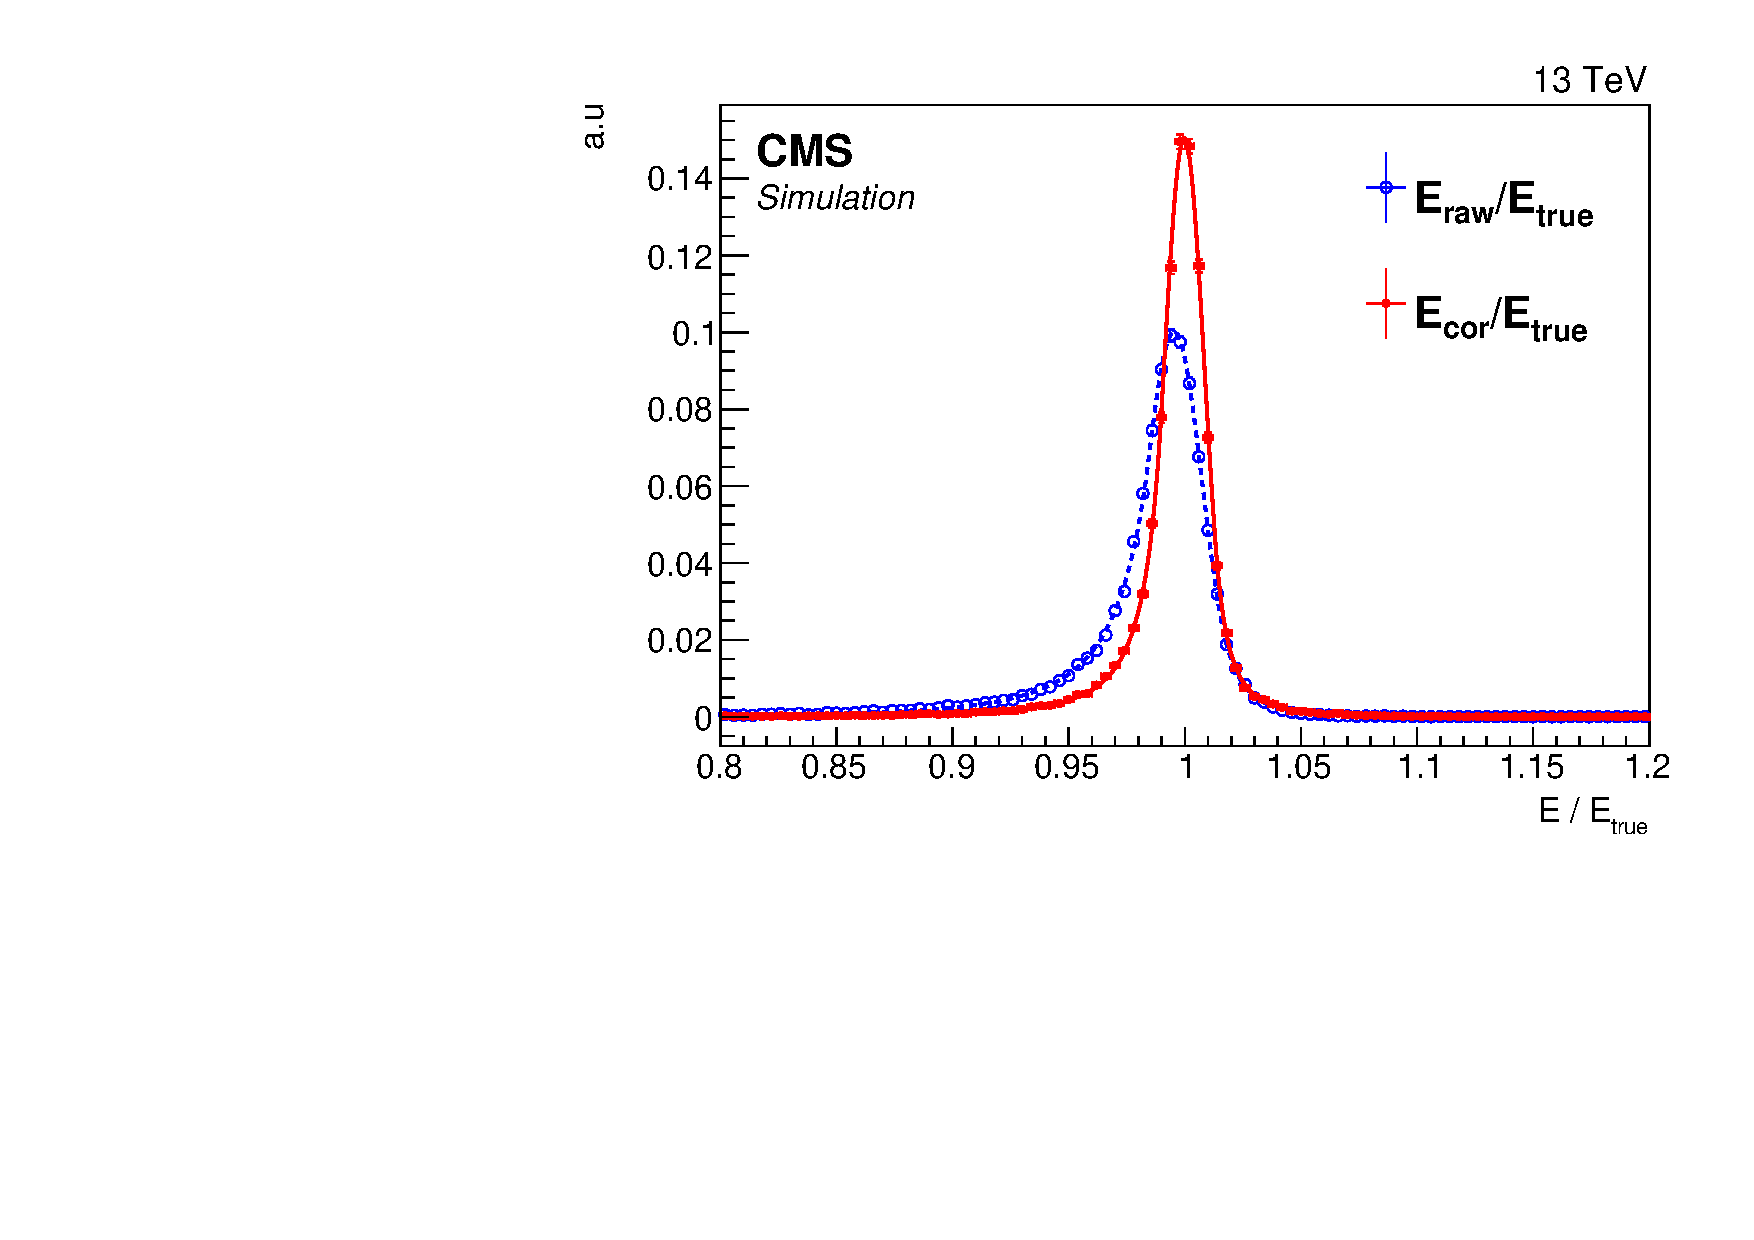
\includegraphics[width=0.45\textwidth]{recoFigures/RegressionEB_Hgg.pdf}
}
  \subfloat[EE]{
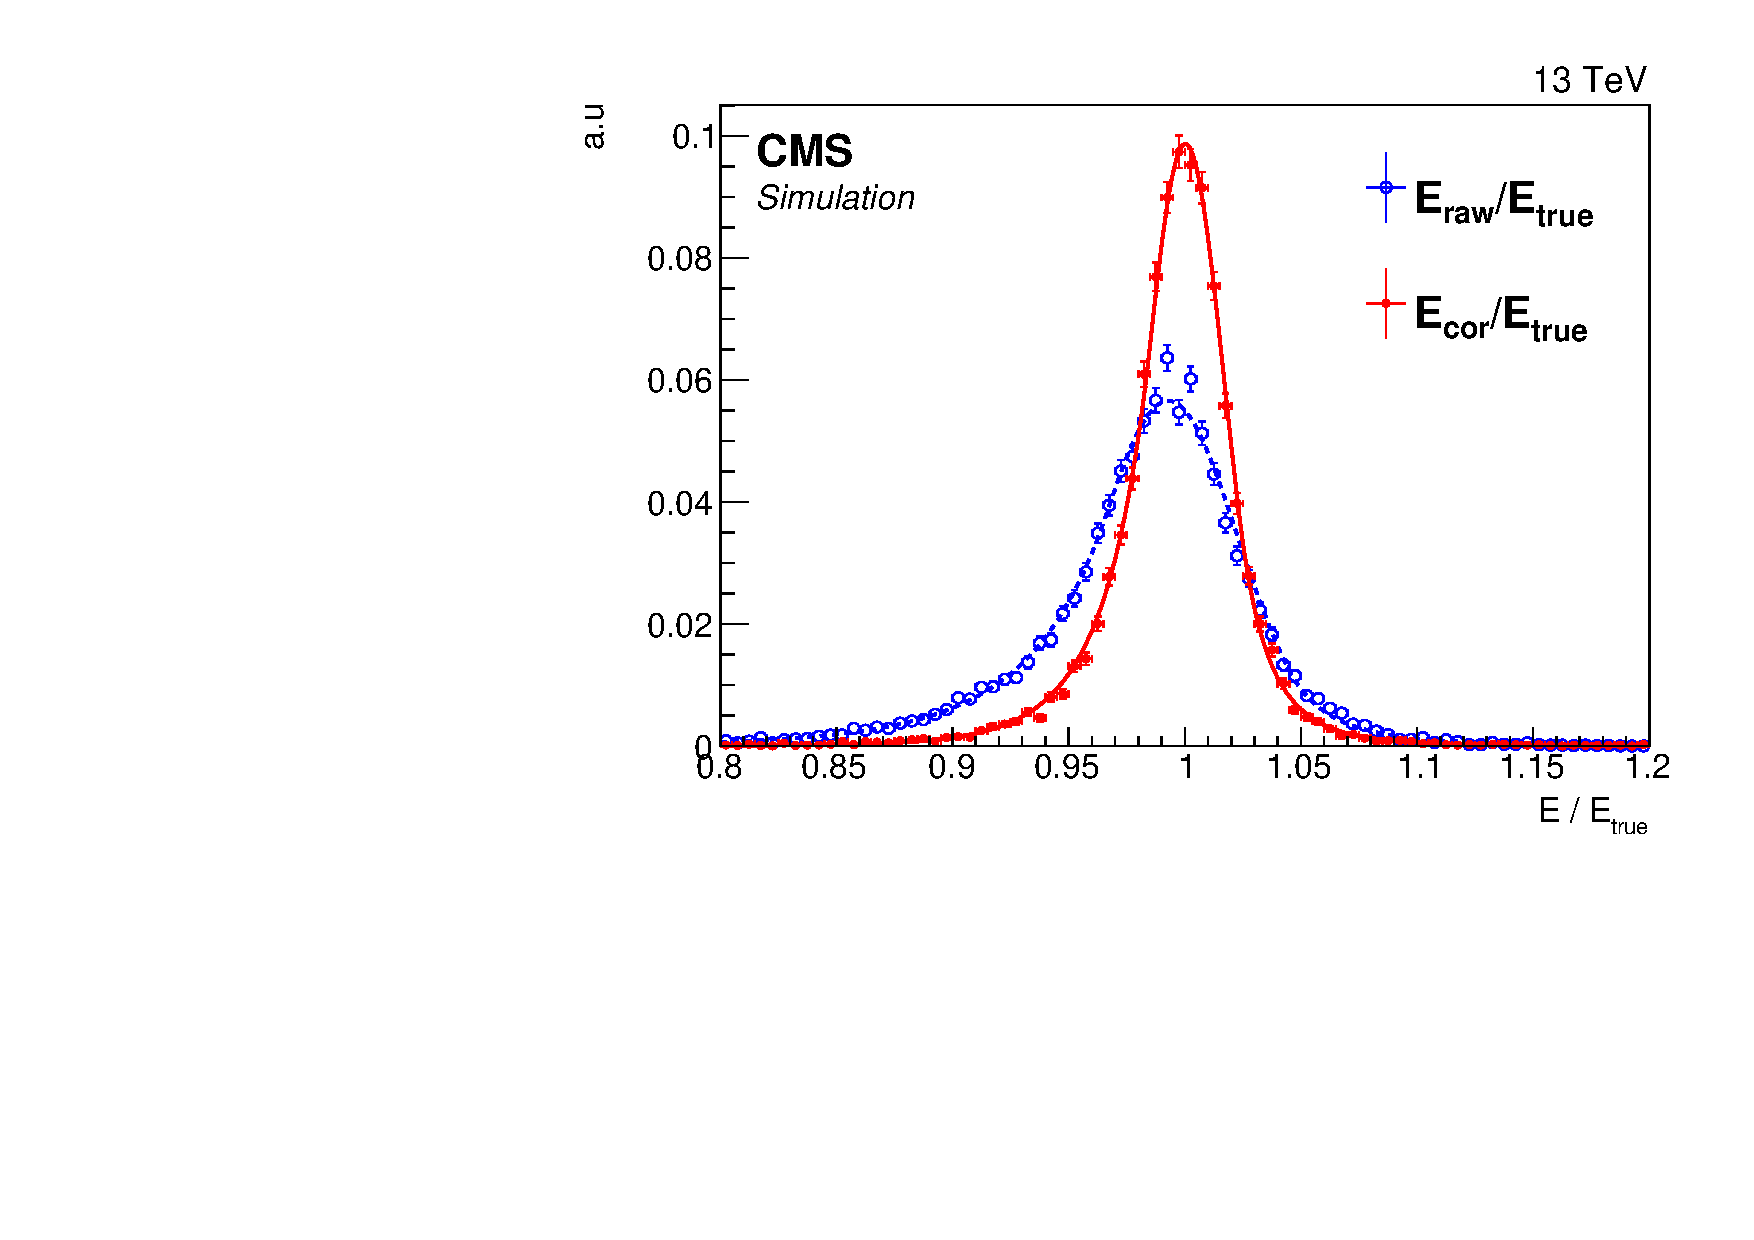
\includegraphics[width=0.45\textwidth]{recoFigures/RegressionEE_Hgg.pdf}
}
\caption{The ratio of the \SC energy and true energy of the simulated photon, shown before the correction is applied ($E_{raw}$) and after the correction is applied ($E_{cor}$), for simulated photons in a sample of \Hgg decays where $\mH=125\GeV$ spearately in the EB and EE. All distributions have been fitted to a DCB function.}

\label{fig:reco:pho_regression}
\end{figure}


\subsection{Photon Pre-selection}
 \label{reco:sec:pho:preselection}

Photon candidates which are to be considered in the \Hgg analysis are required to satisfy certain requirements on their kinematics, shower shapes and isolation. All photon candidates are first required to have an electron veto value of ``false'', and are the grouped into \emph{diphotons} by determining all possible pairs of photons in the event. For each diphoton, the photon with the largest \pT (the \emph{leading} photon) must satisfy $\pT>30\GeV$ while the photon with the second largest \pT (the \emph{sub-leading} photon) must satisfy $\pT>20\GeV$. For diphotons passing this requirement, additional requirements are made on a per-photon basis on the following variables: $\sigma_{i\eta i\eta}$, \HoE, $Iso^{\textrm{PF}\gamma}_{R=0.3}$, $Iso^{\textrm{PF ch. had.}}_{R=0.3}$, $Iso^{\textrm{tracker}}_{0.04<R<0.3}$ and \RNINE. 

The pre-selection is designed to be more stringent than the triggering requirements described in \Sec~\ref{sec:reco:data}, such that the data (which must pass the trigger) and the simulation (for which no triggers are defined) samples inhabit a common phase space.  

The pre-selection efficiency, for all requirements aside from the electron veto, is measured in data and simulation using \Zee events, using a \TagAndProbe technique for different regions of $\eta$ and \RNINE. The results can be seen in \Table~\ref{tab:reco:preslection_eff}. The efficiency of the electron veto was measured separately using a sample of \Zmmg events, and found to be between 96\% and 100\%.

\begin{table}[htbp]
\begin{small}
\begin{center}
\resizebox{\textwidth}{!}{
\begin{tabular}{|l|c|c|c|c|c|c|c|}
\hline
& \multicolumn{ 3}{c|}{DATA} & \multicolumn{2}{c|}{Simulation} & \multicolumn{ 2}{c|}{Ratio} \\
\hline
& Eff. & Stat. Unc. & Syst. Unc. & Eff. & Stat. Unc. & Eff. & Unc. \\
%\hline
%  & \multicolumn{7}{c|}{}\\
\hline
ECAL Barrel; $\RNINE>$0.85 & 0.9451 & 0.0006 & 0.0192 & 0.9374 & 0.0007 & 1.0080 & 0.0192 \\
ECAL Barrel; $\RNINE<$0.85 & 0.8255 & 0.0012 & 0.0119 & 0.8258 & 0.0009 & 0.9960 & 0.0120 \\
ECAL Endcap; $\RNINE>$0.90 & 0.9099 & 0.0008 & 0.0212 & 0.9127 & 0.0010 & 0.9969 & 0.0212 \\
ECAL Endcap; $\RNINE<$0.90 & 0.4993 & 0.0018 & 0.0249 & 0.5024 & 0.0016 & 0.9938 & 0.0250 \\
\hline
\end{tabular}
}
\end{center} 
\end{small}
\caption{Photon pre-selection efficiency (using all requirements aside from the electron veto) measured using \Zee
events in data and simulation with a \TagAndProbe technique.}
\label{tab:reco:preslection_eff}
\end{table}

\subsection{Photon Identification}

In order to separate \emph{prompt} photons (which were prodcued at the \PV) from \emph{fakes} such as misidentified jets, a per-photon \BDT is applied to photon candidates which pass the pre-selection described in \Sec~\ref{reco:sec:pho:preselection}. This \BDT, which is referred to as \PhoIdBdt, is trained on a \gammaJet sample where the signal items are photon candidates which are geometrically matched to a generator-level prompt photon from a \pp interaction, while the background items are composed of photon candidates which have no generator-level photon match, and are therefore likely to have resulted from a misidentified neutral hadron or jet. In both cases, photon candidates are required to pass the event pre-selection. In order to reduce the dependence of the \PhoIdBdt on the kinematics of the photon, the signal items are re-weighted such that their \pT and $\eta$ distributions match those of the background items. The input variables for the \PhoIdBdt are $\sigma_{i\eta i\eta}$, $cov_{i\eta i\phi}$ , $S_{4} $, \RNINE , $\sigma_{\eta} $, $\sigma_{\phi }$, $\sigma_{RR}$, $Iso^{\textrm{PF}\gamma}_{R=0.3}$ , $Iso^{\textrm{PF ch. had.}}_{R=0.3}(\textrm{selected vertex})$, $Iso^{\textrm{PF ch. had.}}_{R=0.3}(\textrm{wrong vertex})$, $\rho$, $\eta_{SC}$ and $E_{SC}$. 

A loose requirement on the output of the \PhoIdBdt is applied to all photons which are considered in the analysis, such that 99\% of the signal photon candidates are kept while a large proportion of background photon candidates are removed. The \PhoIdBdt output score of each photon is then used as a measure of the ``quality'' of each photon, and used as an input for the classification described in \Sec~\ref{}.
The \PhoIdBdt is validated by comparing the output score for data and simulation for diphoton events (\Fig~\ref{fig:reco:photon_id_score_hgg_bkg}) and for $\Zee$ events (\Fig~\ref{fig:reco:photon_id_zee_validation}) where the electron veto requirement was inverted.


\begin{figure}[hptb]
\centering \hspace{0.1cm}
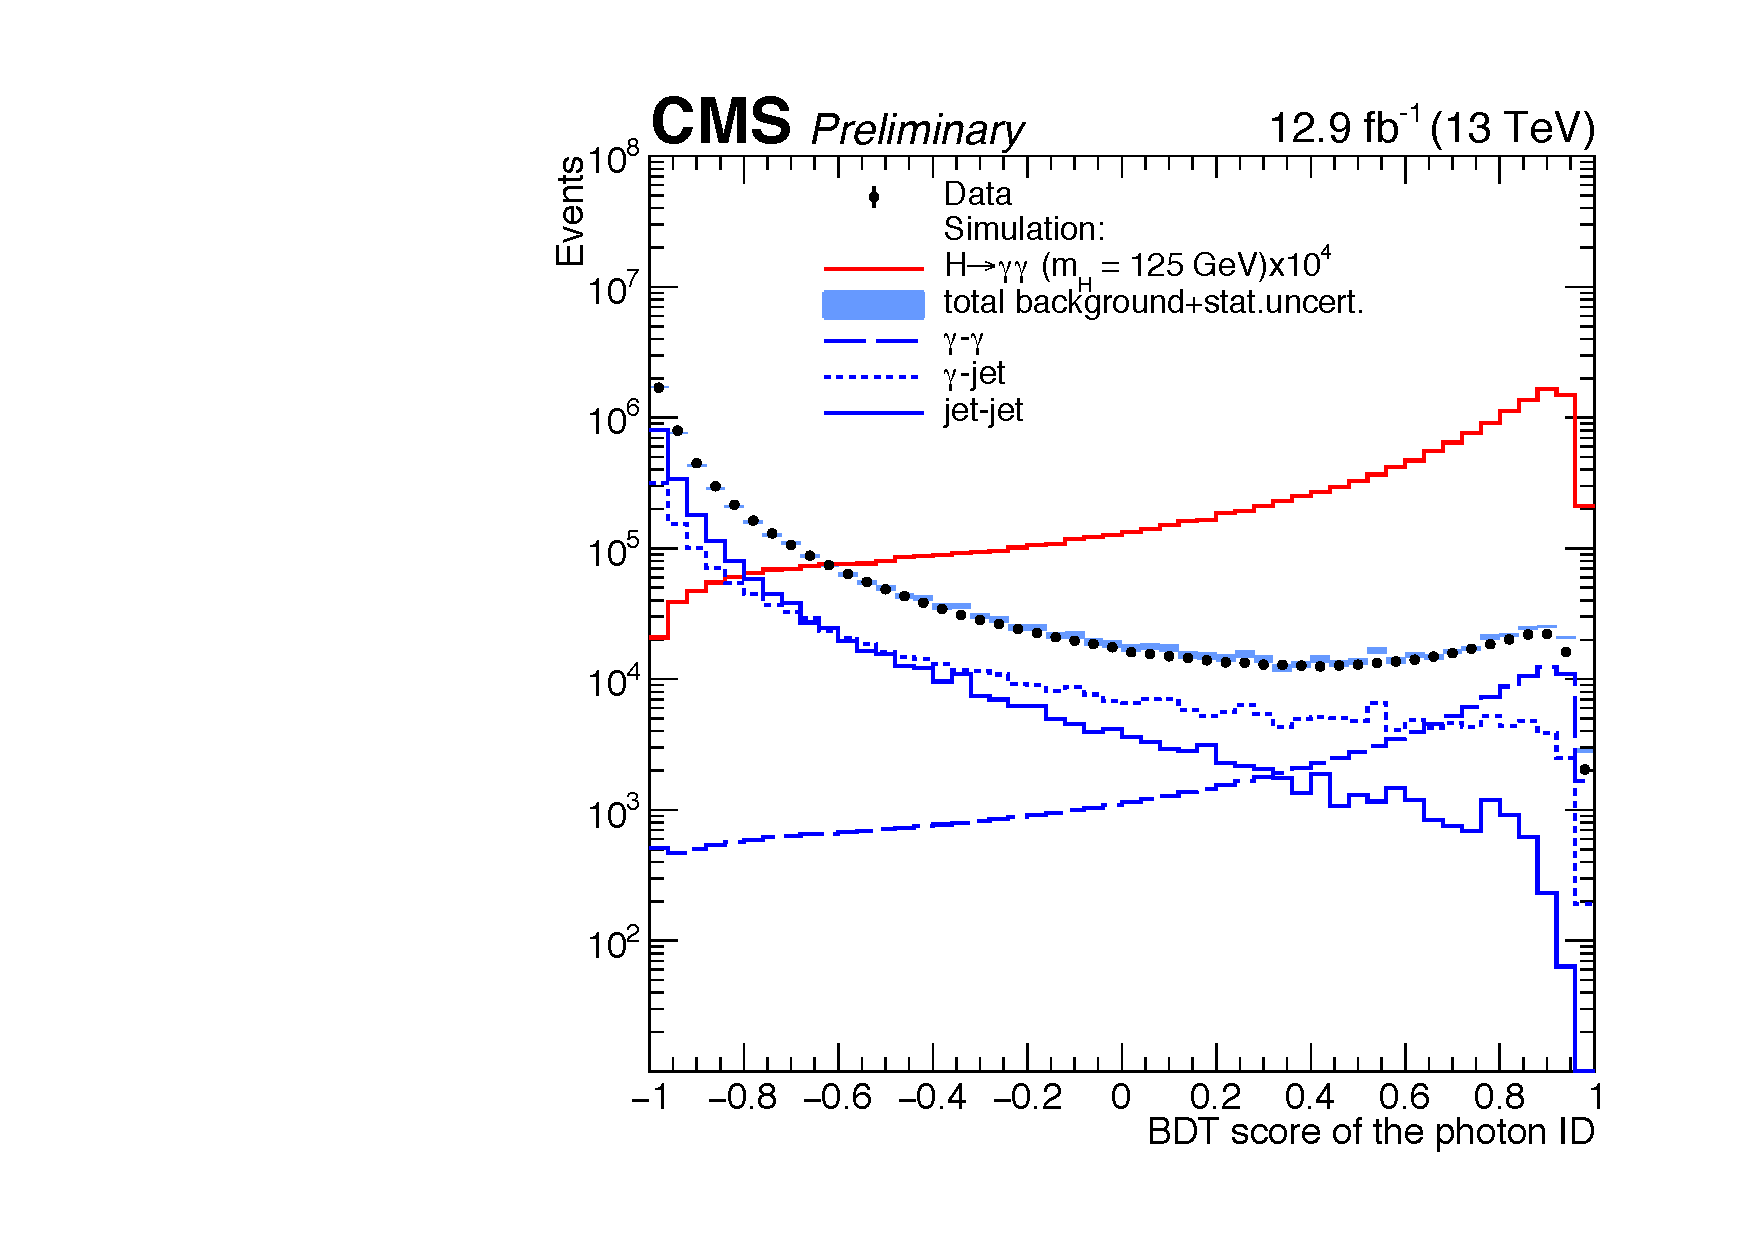
\includegraphics[width=0.59\textwidth]{recoFigures/validation_phoID_ICHEP_4sideTicks.pdf}
\caption{
The distribution of the \PhoIdBdt output score for the lower-scoring photon in each diphoton pair in the range $100 < m_{\gamma \gamma} < 180\GeV$ for data and simulation. The simulation is composed of signal (\Hgg photons with $\mH=125\GeV$) and background, which has been split into prompt-prompt ($\gamma$-$\gamma$), prompt-fake ($\gamma$-$\textrm{jet}$) and fake-fake ($\textrm{jet}$-$\textrm{jet}$) components. The sum of the background components has been scaled to match the number of events in data.}
\label{fig:reco:photon_id_score_hgg_bkg}
\end{figure}

\begin{figure}[hptb]
\centering 
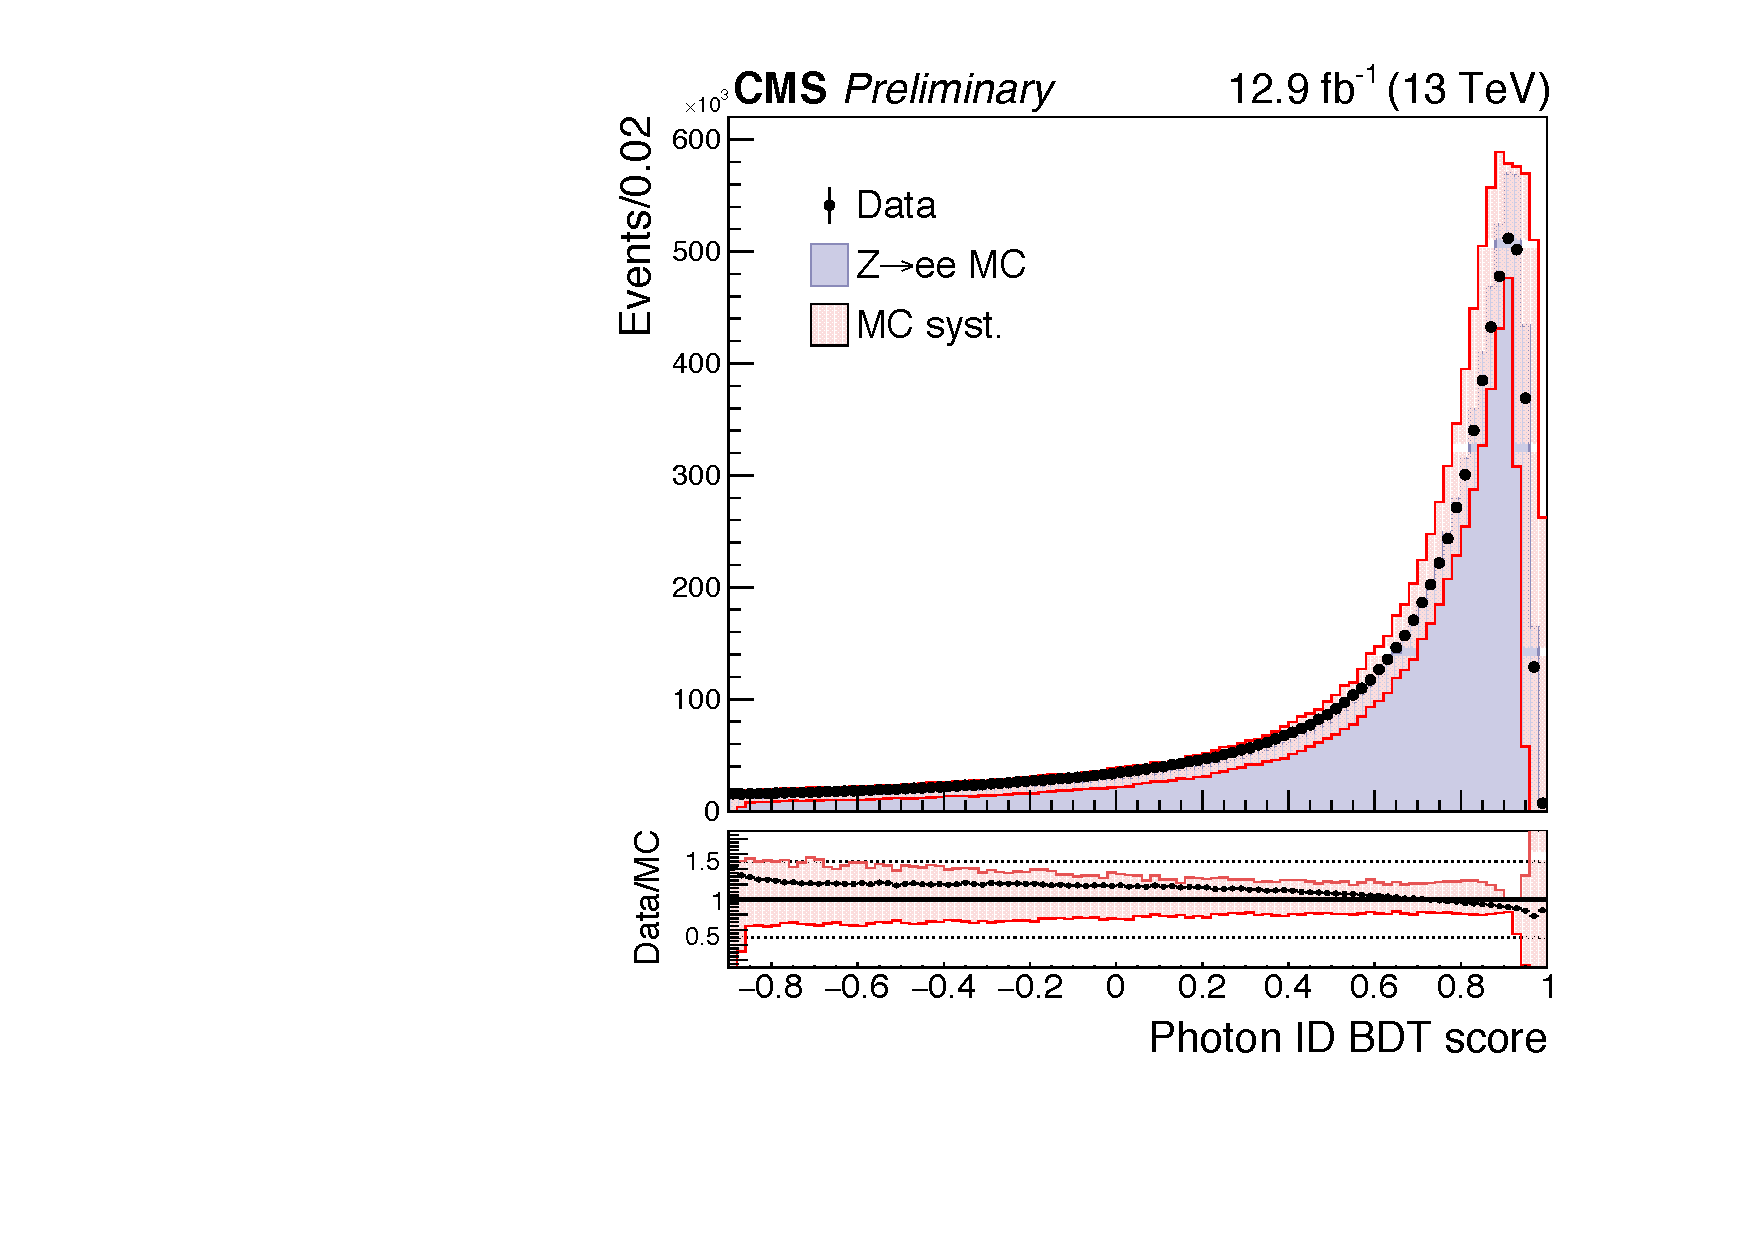
\includegraphics[width=0.68\textwidth]{recoFigures/idmva_syst_combined.pdf}
\caption{ The $\text{BDT}_{\gamma\text{ ID}}$ output score for \Zee events in data and simulation (labelled MC), where 
the electrons are reconstructed as photons with the electron veto requirement inverted.}
\label{fig:reco:photon_id_zee_validation}
\end{figure}


\section{Vertex Reconstruction}
\label{reco:sec:vertex}

\subsection{Vertex Identification}
As was discussed in \Sec~\ref{reco:sec:intro}, the determination of the location of Higgs decay is an important step in the reconstruction of \Hgg events, as it impacts the calculation of the invariant mass of diphoton system. Studies performed during the analysis of the \RunI dataset showed that if the selected vertex is within 1\cm of the true vertex location in the $z$-direction, then the impact of the opening angle on the mass resolution is negligible. Conversely, failing to identify the vertex within 1\cm leads to a degradation of the mass resolution of order 1\GeV. %CITATION NEEDED?

Since the \CMS \ECAL is composed of a single layer of crystals, it cannot be used to point towards the vertex location. %Furthermore, unless a photon undergoes pair conversion, it does not leave any tracks in the tracker. 
None the less, it is possible to exploit tracks recoiling from the diphoton system and the tracks of any electrons resulting from pair conversion to help determine the location of the vertex.
The first step is to produce a list of candidate vertex locations by considering all the tracks recorded in the tracker and grouping them into common points of origin by determining their closest point of approach to the beam-line.

A per-vertex \BDT is used to determine which of the candidate vertices is most likely to be the point of origin of the Higgs boson decay. This \BDT is refereed to as \VtxIdBdt. The set of input variables is listed below, where $N_{tracks}^{vtx}$ is the number of charged \PF candidates associated with a given vertex, $\vec{\pT}^i$ is the transverse momentum of the $i^{\textrm{th}}$ candidate and $\vec{\pT}^{\gamma\gamma}$ is the transverse momentum of the diphoton system :
\begin{itemize}
\item the sum of squared transverse momenta of all tracks, $\sum_{i=0}^{N_{tracks}^{vtx}} | \vec{\pT}^{i} |^2$;
\item the transverse momentum balance,  $\sum_{i=0}^{N_{tracks}^{vtx}} (- \vec{\pT}^i \cdot \frac{\vec{\pT}^{\gamma\gamma}}{|\vec{\pT}^{\gamma\gamma}| })$;
\item the transverse momentum asymmetry,  $\frac{(|\sum_{i=0}^{N_{tracks}^{vtx}} \vec{\pT}^i| - |\vec{\pT}^{\gamma\gamma}|)}{(|\sum_{i=0}^{N_{tracks}^{vtx}} \vec{\pT}^i| + |\vec{\pT}^{\gamma\gamma}|)}$.
\end{itemize}

Two additional variables are also considered if one of the two photons has converted into an $\Pep\Pem$ pair, where additional information is available to help identify the vertex:
\begin{itemize}
\item the number of converted photon candidates in the event;
\item the pull $|z_{vertex} - z_{conv}|/\sigma_{z_{conv}} $, where $z_{vertex}$ and $ z_{conv}$ are the $z$-components of the positions of the reconstructed vertex under consideration  and the position of the vertex extrapolated from the conversion tracks respectively, and $\sigma_{z_{conv}} $ is the uncertainty on the extrapolated vertex position.
\end{itemize}

The \VtxIdBdt was trained using simulated Higgs boson events with $\mH=126\GeV$, where event from each productions mode were weighted by their respective cross-section. The signal items are the vertices where the Higgs boson decay occurs at generator level. Any vertex in the sample which is not associated with a Higgs boson decay is treated as a background item. The training samples are re-weighted to account for the fact that the width of the \emph{beamspot} (the distribution of the number of reconstructed vertices as a function of longitudinal position) in data and simulation is not the same: this width is modelled as 5.1\cm in simulation but is measured to be 3.6\cm in the data samples considered in this analysis. The re-weighting is performed as a function of the distance $\Delta z$ between the true vertex and the selected vertex, such that the distribution of $\Delta z$ after the re-weighting in simulation after the re-weighting matched the expected $\Delta z$ distribution in data, which is the beamspot width in data multiplied by a factor of $\sqrt{2}$.

The \VtxIdBdt was validated for unconverted photos using \Zmumu events in data and simulation. After determining the true vertex of the decay from the muon tracks, the events were re-reconstructed removing the muon tracks to mimic the decay of the Higgs boson to photons.  For converted photons, the \VtxIdBdt was validated using a similar technique with \gammaJet samples, where the true vertex is obtained from the tracks associated with the jet, and the events are re-reconstructed removing the tracks associated with the jet to mimic a diphoton system. The vertex-finding effiencies as a function of \pT and as a function of the number of vertices in the event can be seen in \Fig~\ref{fig:reco:vtxidbdt_eff} and \Fig~\ref{fig:reco:vtx_id_eff_zmumu_validation}. %The data sample was obtained by triggering on isolated muon tracks with $\pT > 27\GeV$, requiring tight identification criteria for both muons, and selecting events where the invariant mass of the dimuon system was between 70\GeV and 110\GeV. A simulated sample of \Zmumu events is used for this study, where the events have been re-weighted such that their \PU distribution matches that of the data and the beamspot re-weighting discussed in \Sec~\ref{} is applied. The differences between the data and simulation are used to estimate the systematic uncertainties associated with the choice of vertex. %and \gammaJet
\begin{figure}
\begin{center}
%\includegraphics[width=0.45\linewidth]{vtxIdFig/eff_pt_Zmumu.pdf}
%\includegraphics[width=0.45\linewidth]{vtxIdFig/eff_nVtx_Zmumu.pdf}
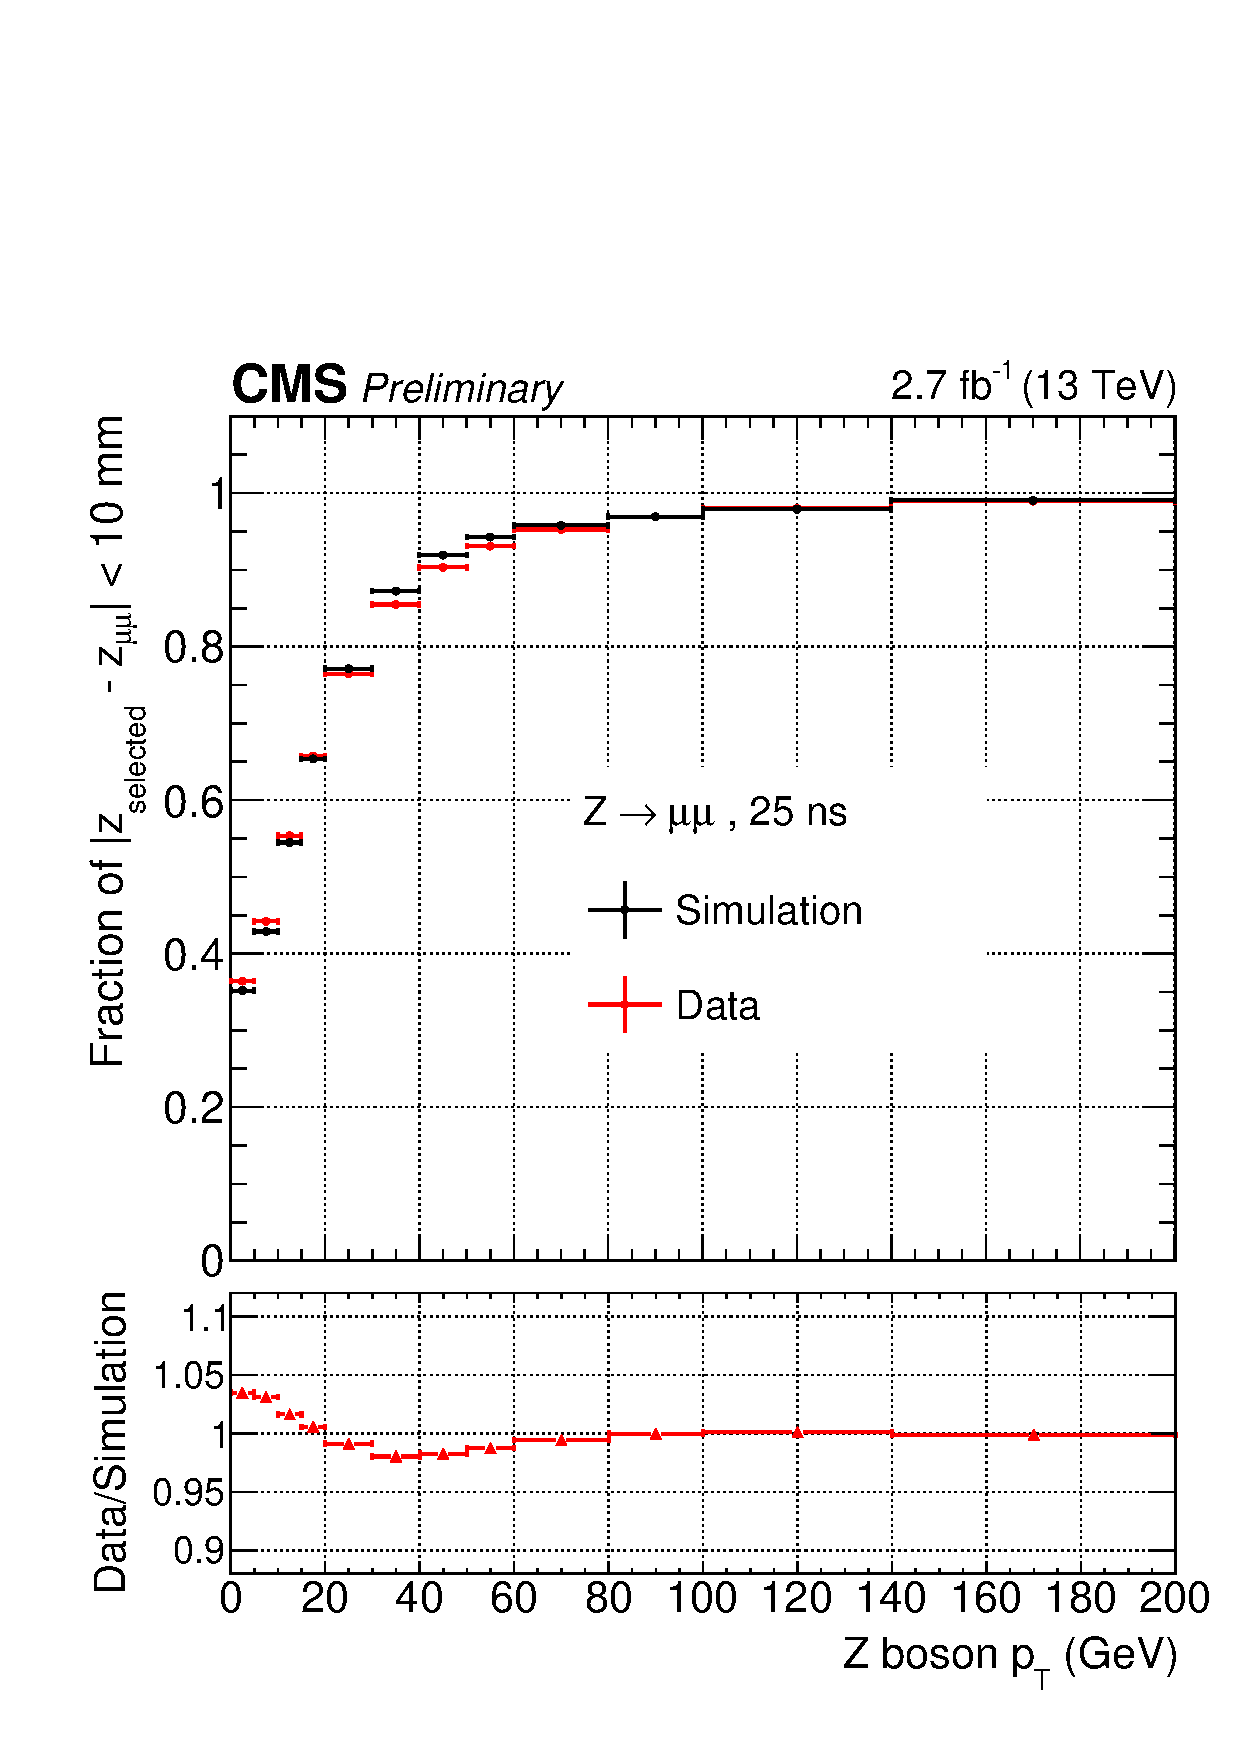
\includegraphics[width=0.45\linewidth]{recoFigures/last_Zmumu_eff_vs_pt_76X_VariableBins_ChangeHLT.pdf}
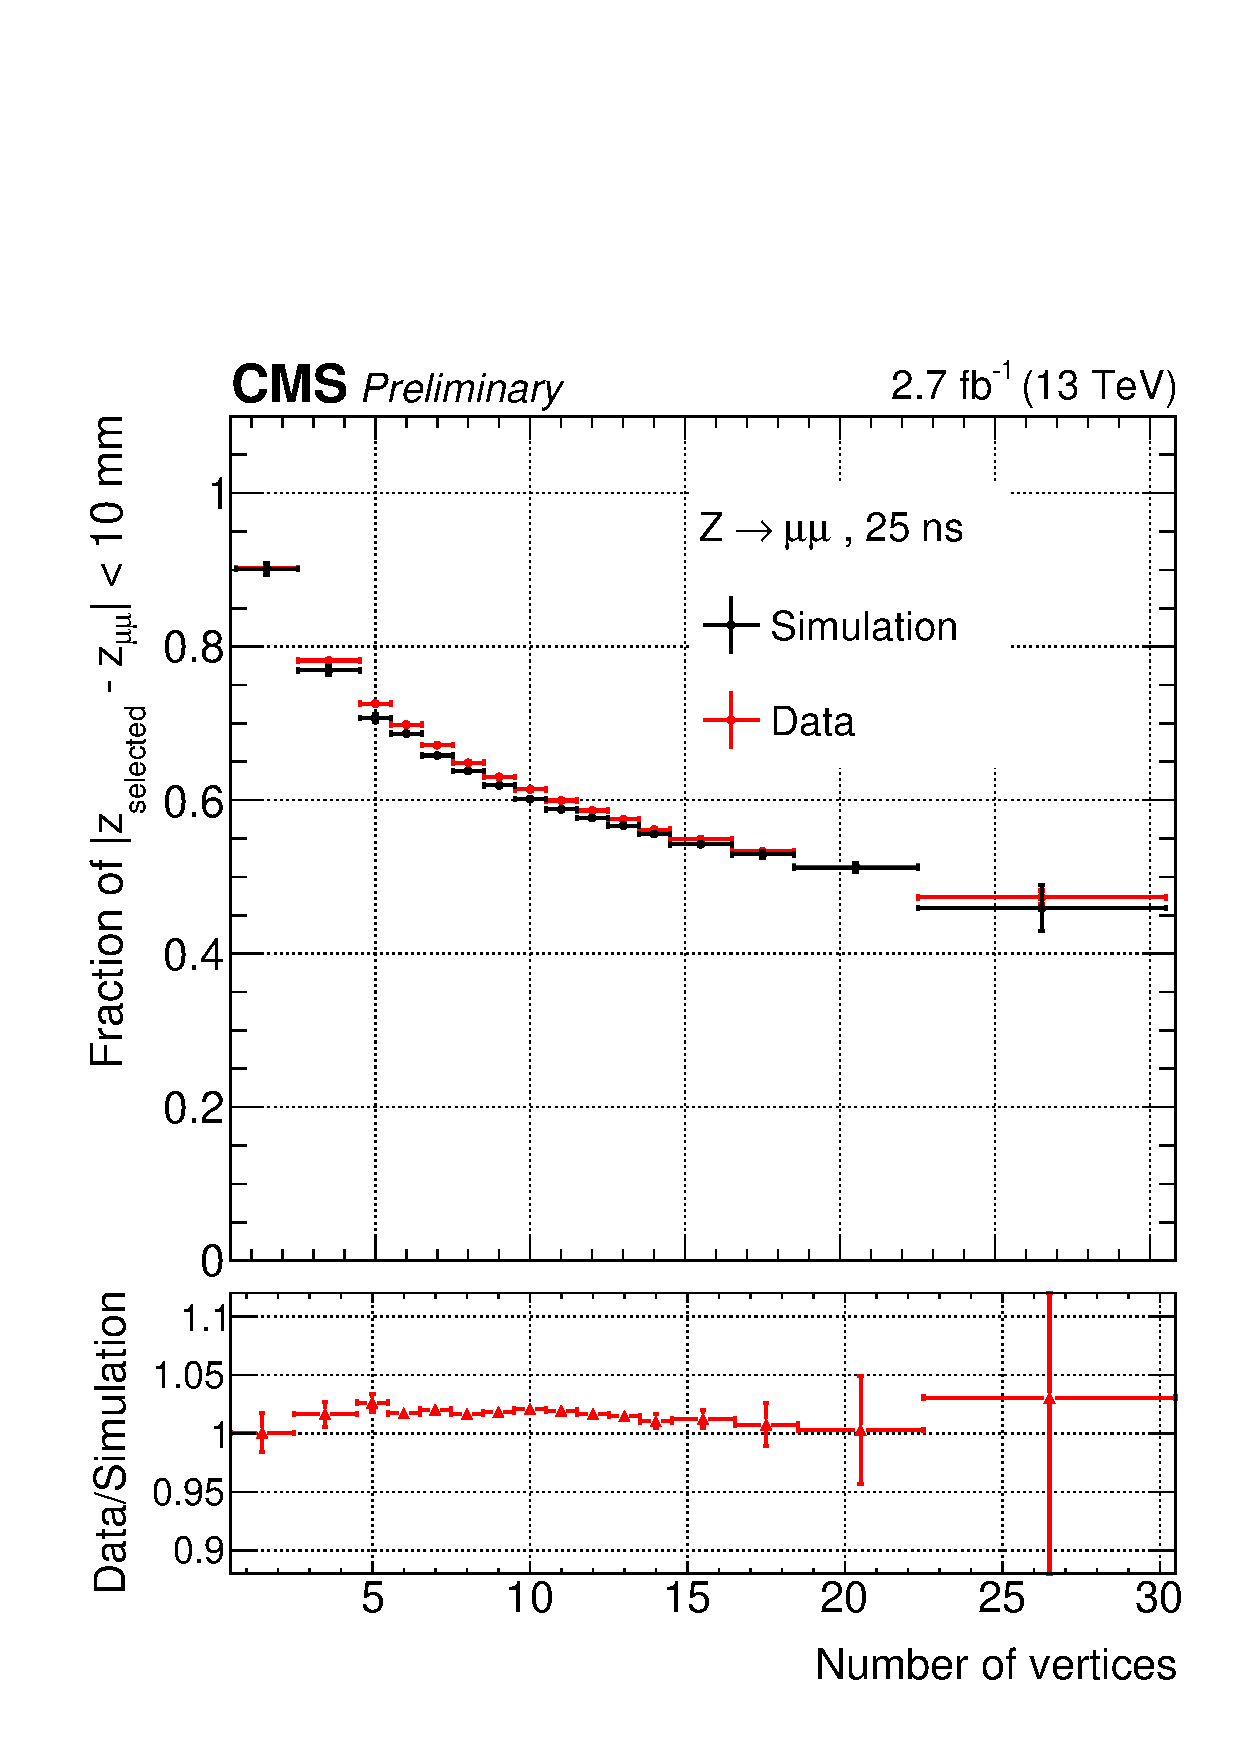
\includegraphics[width=0.45\linewidth]{recoFigures/last_Zmumu_eff_vs_nVtx_76X_VariableBins_ChangeHLT.pdf}
\caption{The efficiency of selecting a vertex within 1\cm of the true vertex in \Zmumu events, as a function of the \pT of the $\PZ$-boson(left) and as a function of the number of vertices (right) in the event.}
\label{fig:reco:vtx_id_eff_zmumu_validation}
\end{center}
\end{figure}

\begin{figure}
\begin{center}
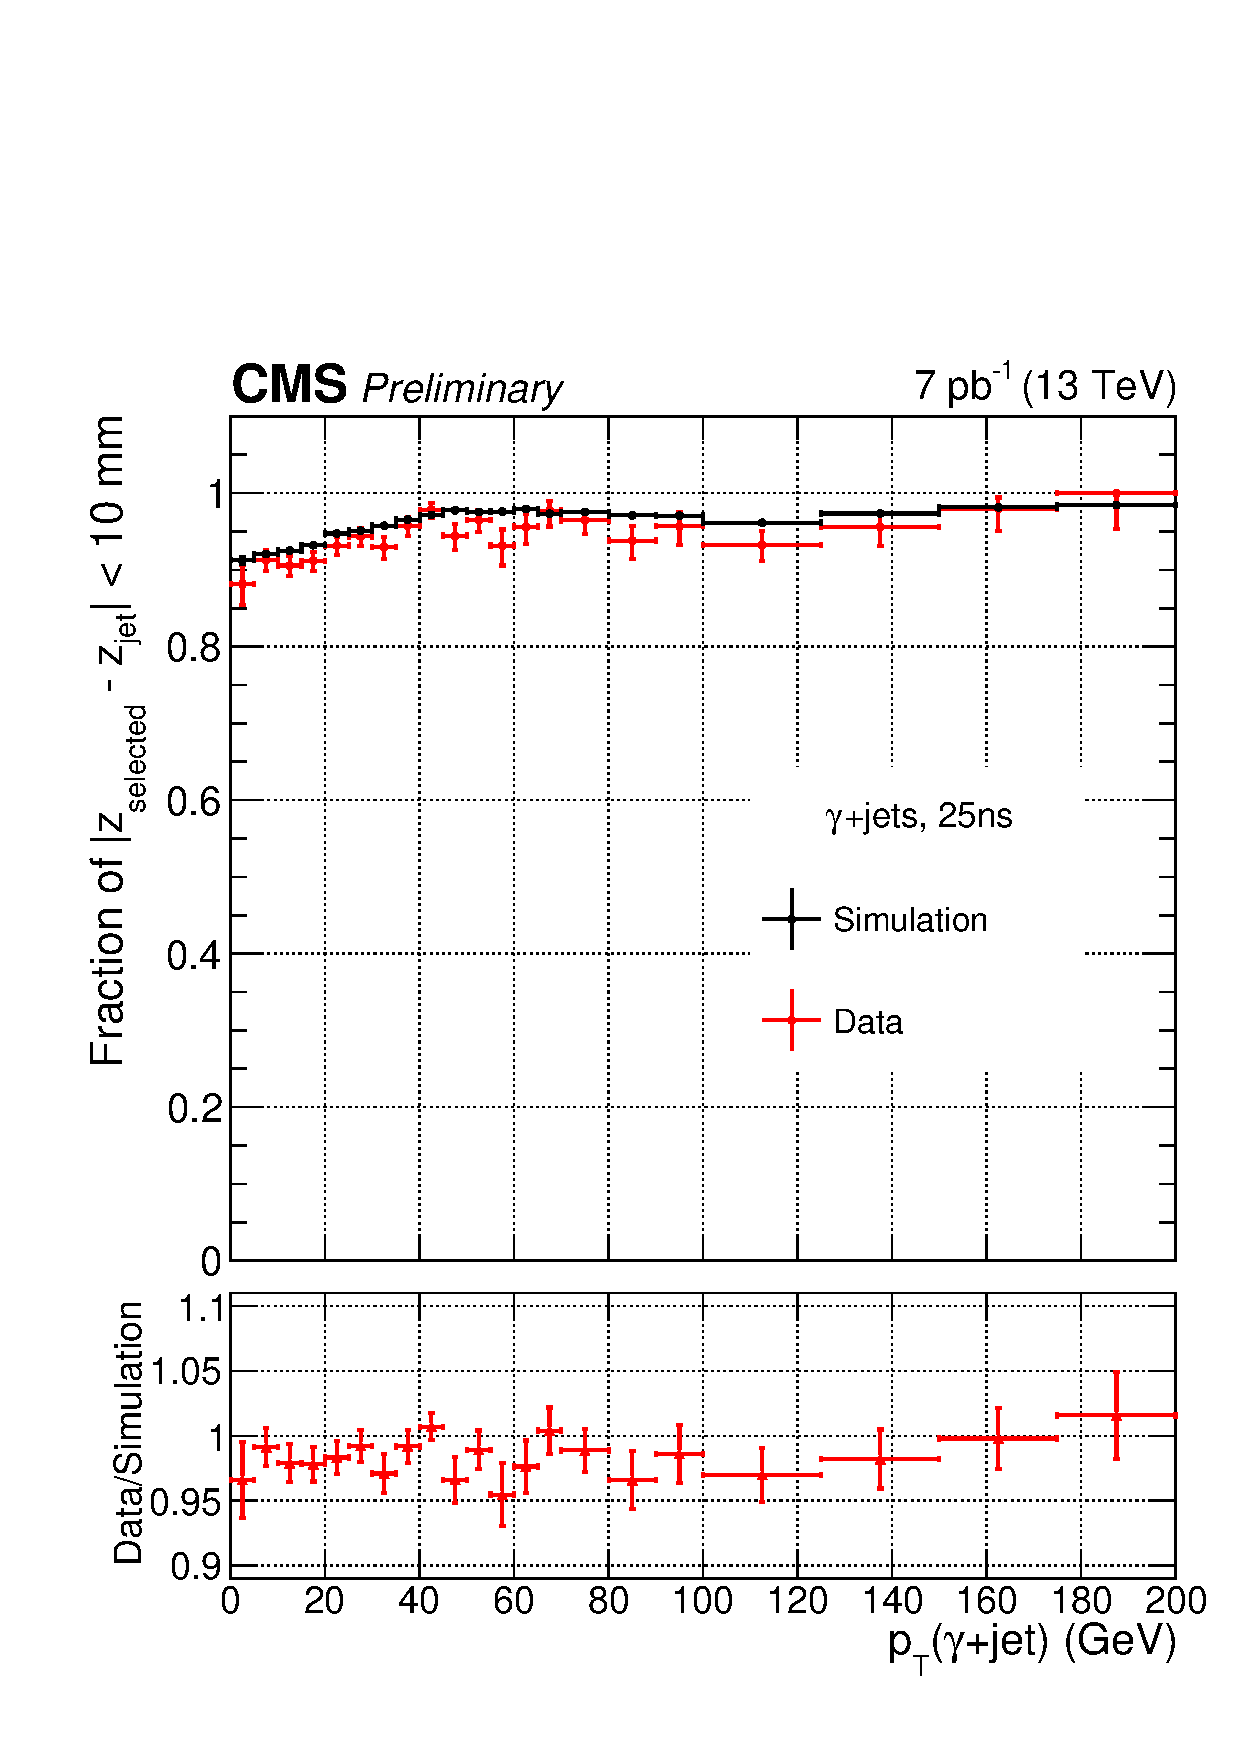
\includegraphics[width=0.45\linewidth]{recoFigures/last_gamma_jets_eff_vs_pT.pdf}
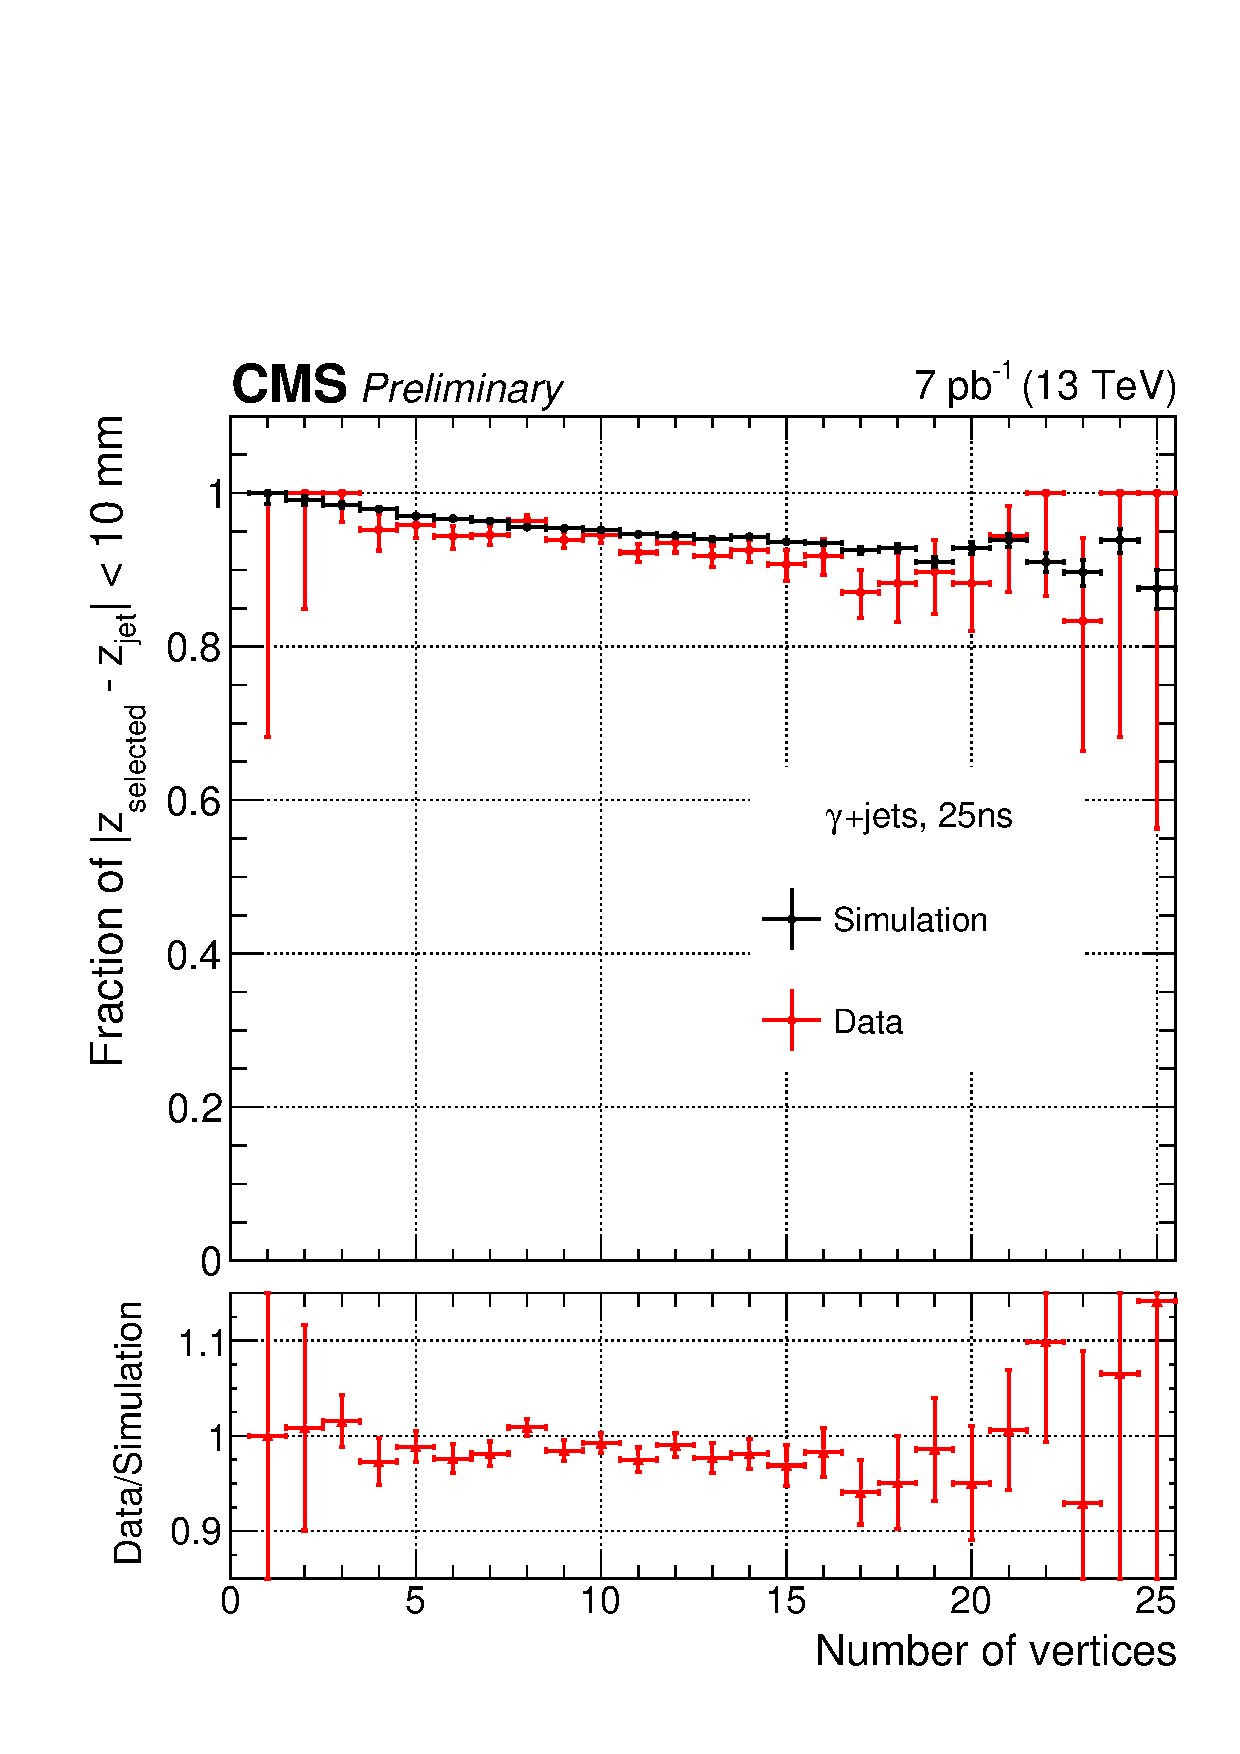
\includegraphics[width=0.45\linewidth]{recoFigures/last_gamma_jets_nVtx.pdf}
\caption{The efficiency of selecting a vertex within 1\cm of the true vertex in \gammaJet events, as a function of the \pT of the \gammaJet systen (left) and as a function of the number of vertices (right) in the event.}
\label{fig:reco:vtx_if_eff_gjet_validation}
\end{center}
\end{figure}


The efficiency of the \VtxIdBdt to select the right vertex within 1\cm of the true one was estimated with signal events where $\mH=125\GeV$. The results are shown as a function of the number of vertices in the event and as a function of \pT, these can be seen on \Fig~\ref{fig:reco:vtxidbdt_eff}. The average efficiency is of the order of 80\%. 

\begin{figure}[h]
\centering
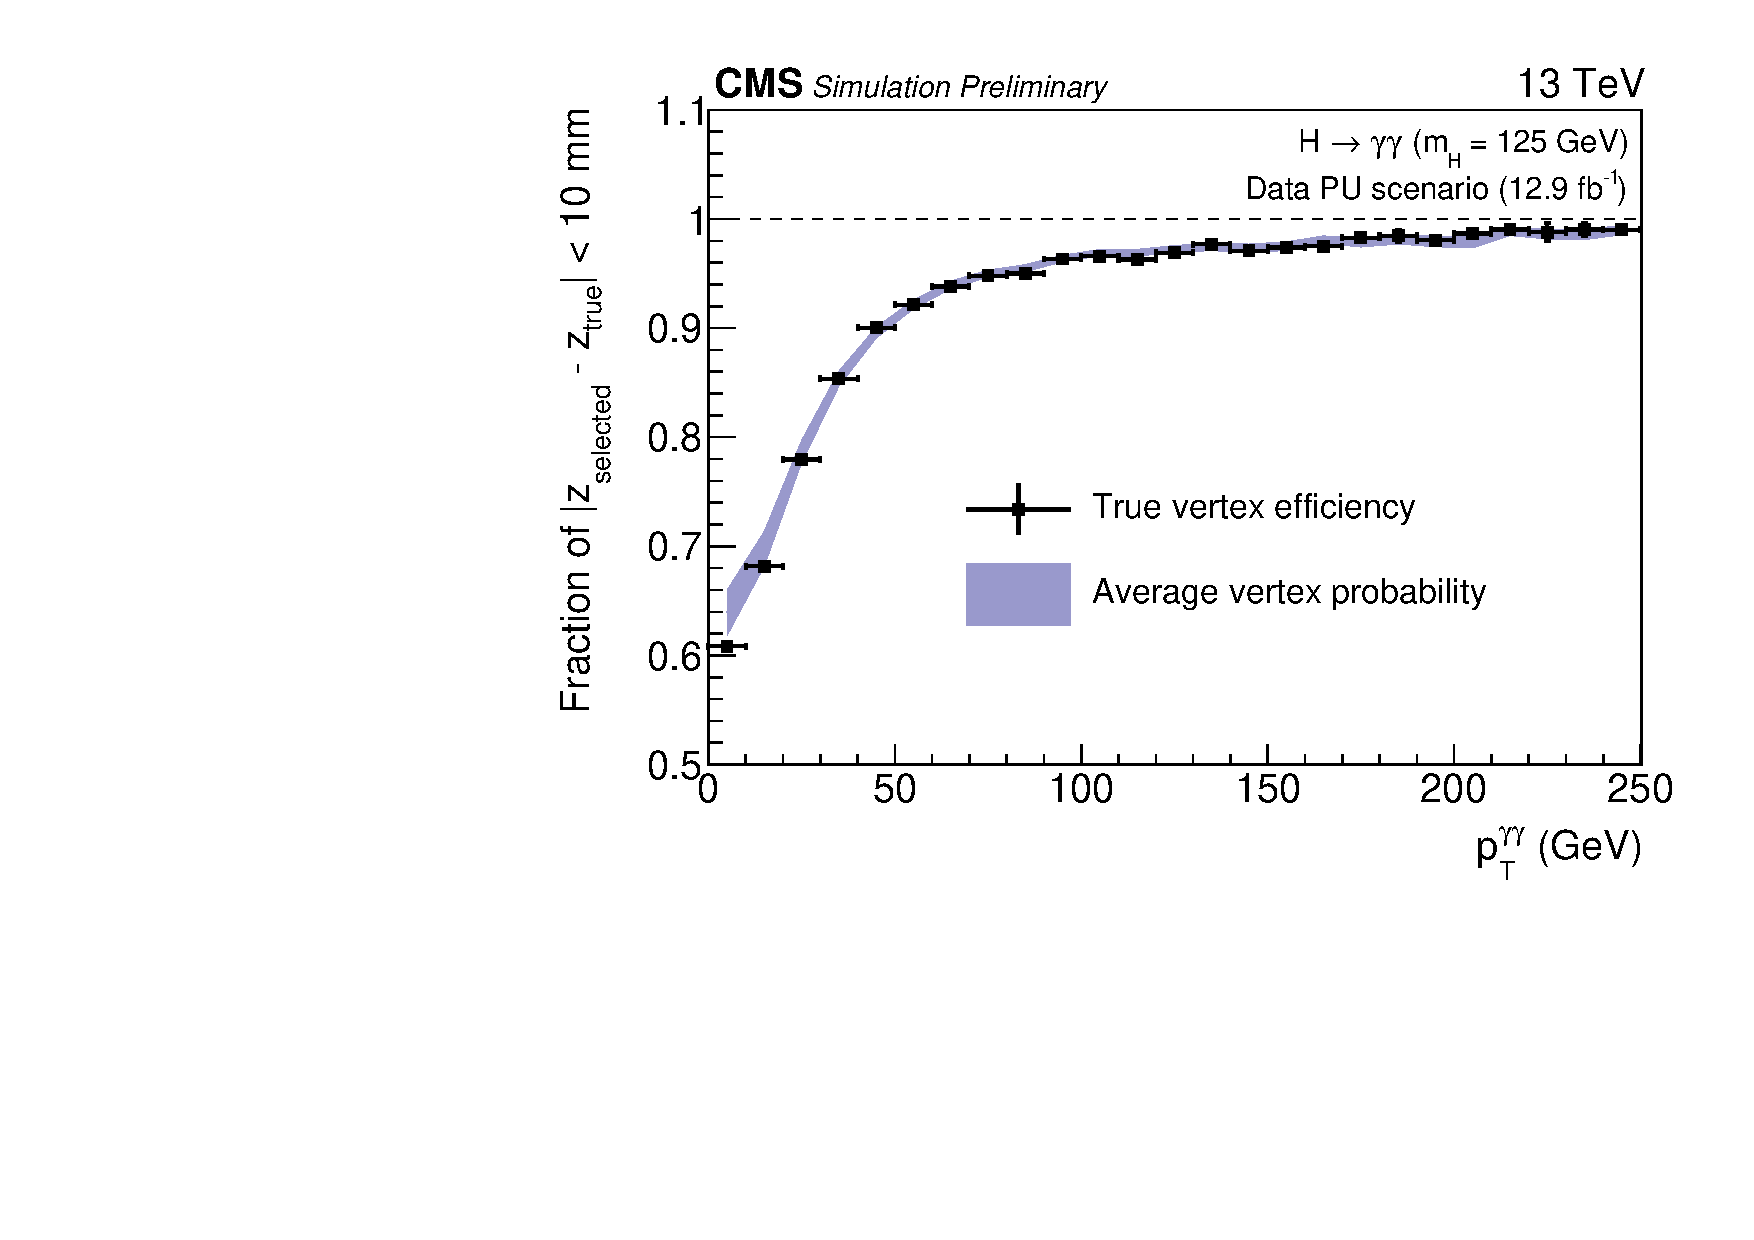
\includegraphics[width=0.7\textwidth]{recoFigures/Pt2016PU125BSReweighted12.pdf}
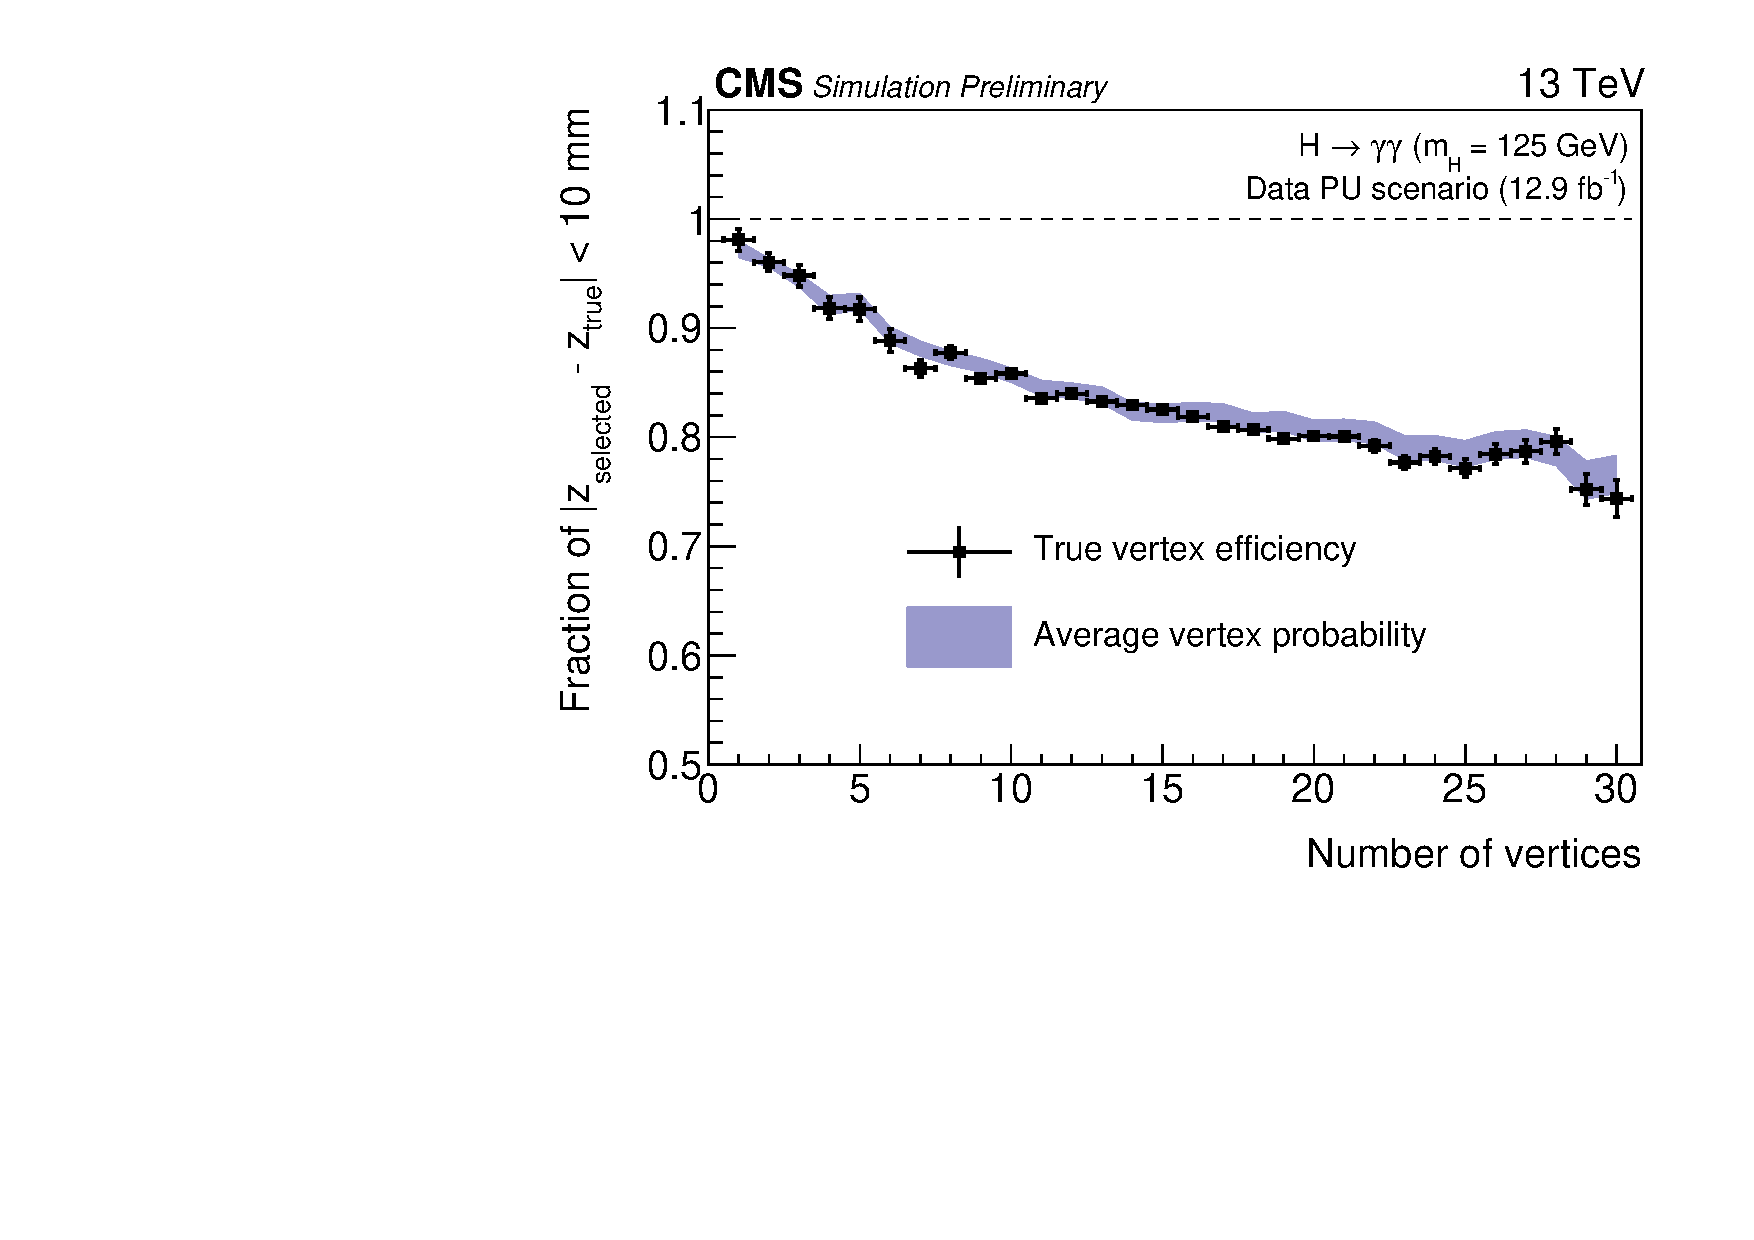
\includegraphics[width=0.7\textwidth]{recoFigures/Nvtx2016PU125BSReweighted12.pdf}
\caption{The efficiency to select a vertex within 1\cm of the true vertex in simulated \Hgg events as a function \pT and the number of vertices in the event. The estimated probability that the vertex was chosen within 1\cm is super-imposed. The uncertainty on the vertex-finding probability was determined using \Zmumu events. The simulation was re-weighted such that the distribution if the number of vertices and the width of the interaction region matched in data and simulation. }
\label{fig:reco:vtxidbdt_eff}
\end{figure}

\subsection{Correct Vertex Probability}

If the chosen vertex is over 1\cm away from the true one, the invariant mass resolution is dominated by the uncertainty on the vertex position. It is therefore desirable to have a per-event estimate of how likely it is that the vertex was chosen within 1\cm of the true one. This is referred to as the \emph{correct vertex probability}. This information is used to categorise events by sensitivity, as described in \Sec~\ref{}.

The estimate of the per-event vertex probability is obtained using a \BDT, which is labelled \VtxProbBdt. The input variables for this \BDT are:

\begin{itemize}
\item the number of reconstructed vertices in the event;
\item the \pT of the diphoton system;
\item the output scores of the three vertices ranked highest by the \VtxIdBdt;
\item the distance in the $z$-direction between the first- and second-highest ranked vertices;
\item the distance in the $z$-direction between the first- and third-highest ranked vertices;
\item the number converted photons in the diphoton. 
\end{itemize}

The correct vertex probability is parametrized by a $4^{th}$-order polynomial as a function of \VtxIdBdt output score. This is done separately for converted and unconverted photons. The estimated correct vertex identification probability is shown alongside the vertex efficiency measured in simulation of \Fig~\ref{fig:reco:vtxidbdt_eff}. The \VtxProbBdt was validated using \Zmumu and \gammaJet events analogously to the \VtxIdBdt. 

\section{Other objects} 
\label{reco:sec:other}
\subsection{Electrons}

In the study of the \Hgg decay, electrons are used in two ways. First, they are used to validate reconstruction algorithms using \Zee events. Second, they are used for the categorisation of \Hgg events where the Higgs boson events was produced by the \VH mechanism. Candidate \PF electrons are reconstructed from \ECAL deposits matched to a track in the tracking system. Electron candidates can either be reconstructed starting from \ECAL deposits which are then matched to tracks (in which case they are called \emph{ECAL-driven} electrons), or conversely starting from tracks whcih are then associated with matching \ECAL deposit (these are \emph{tracker-driven} electrons). Typically, energetic and isolated electron candidates will be reconstructed as \ECAL-driven, while low-energy $<10\GeV$ electrons will be reconstructed as tracker-driven. Electrons from both seeding algorithms are eventually grouped together to form the set of \PF electron candidates. The electrons which are used in this thesis originate from \PWpm or \PZ decays, and hence are mostly ECAL-driven.

The ECAL-seeded electrons are obtained via a procedure analogous to that described for photons in \Sec~\ref{reco:sec:photons}, but with the additional step of associating a track based on geometrical requirements. Candidate tracks are obtained by from tracker hits which are within some window in $z$ and $\phi$ around the \SC position. The tracks are fitted with a special algorithm which takes into account the change in direction caused by the emission of bremsstrahlung. The \SC is associated to the track whose extrapolated position in the \ECAL is nearest to the energy-weighted position of the \SC, but requiring that the distance in the $\eta$-direction ($\phi$-direction) be no more than $0.02$ (0.15). The energy of electrons is obtained from the \SC energy, where the final energy correction $F_{SC}$ is obtained using a \BDT method analogous to that described in \Sec~\ref{sec:reco:photon:phoenergybdt}, but specially trained for electron candidates.

\subsection{Muons}

In this analysis, Muons are used for the validation of reconstruction algorithms using \Zmmg events, and also for the selection of Higgs boson which were produced by the \VH mechanism. Muons are constructed by geometrically matching tracks reconstructed independently in the tracking system and in the muon chambers. Muon candidates must have some hits in both sub-detectors to qualify as \PF muons: this helps to avoids cases where cosmic rays or muons produced in jets are mis-reconstructed as prompt muons from the \PV~\cite{MuonReco}.  

\subsection{Jets}

Jets are collections of collimated particles originating from the decay of quarks or gluons. In the \Hgg analysis, jets are used to identify events where the Higgs boson was produced by the \VBF process. 
Jets are reconstructed using the \antiKt clustering algorithm~\cite{antiKt} from \PF candidates, using a cone of radius $R=0.4$. Jets originating from \PU can sometimes overlap with jets which originate from particles produced at the \PV. To mitigate this effect, \PFCHS is used. In this scheme, the \PF charged hadron candidates which are associated to a vertex other than the vertex selected by the procedure described in \Sec~\ref{reco:sec:vertex} are ignored during the clustering. %Events can have multiple possible photon pairs ans since each photon pair is associated with a vertex, the event can have potentially multiple possible selected vertices. The collection of jets is therefore reclustered using the \PFCHS under all possible selected vertex scenarios. 
Since the tracker acceptance is $|\eta|<2.5$, no \PF charged hadron candidates are available outside this range, so \PFCHS has no effect. For the jets reconstructed outside this region, but still in acceptance, a different \PU mitigation technique is used using a selection on the width of the jet. The width of the jet is described by the variable $\RMS= \sum_{\text{PF candidates}}\pT^2 \Delta R^2/ \sum_{\text{PF candidates}}\pT^2  $, where $\Delta R$ is the distance between the \PF candidate and the jet axis from the clustering cone. Jets must have $\RMS<0.03$ to pass the \PU mitigation requirement. Finally, all jets are required to be within  $|\eta|<4.7$.

Parametric corrections to the energy of the jets is made to account for the followign effects:
\begin{itemize}
\item the additional energy of \PF neutral hadrons from \PU which are clustered into jets; 
\item the non-uniformity of the detector response;
\item the difference between data and simulation in \gammaJet and $\PZ+\text{jet}$ events.
\end{itemize}


\subsection{Missing energy}

Particles which do not leave any deposits in the detector, such as neutrinos, still need to be reconstructed in order to identify decays from $\PWpm$ bosons, for example when identifying Higgs boson decays originating from the \WH production mode. Such particles are reconstructed by identifying \MET, which is the amount of energy taken away by these particles as they leave the detector. \MET is calculated by considering the magnitude and direction of \pT required to balance all the jets and \PF objects in an event.


